%\thispagestyle{empty}
\chapter{Экспериментальное исследование волновых движений на поверхности и в толще жидкости} \label{chapt2}

\section{Введение} \label{sect2_1}
В связи расширением разведки и добычи нефти и газа в шельфовой зоне океанов и морей большую важность приобрела информация об экстремальных значениях ветра и волн, поскольку буровые установки и платформы должны эксплуатироваться при любых погодных условиях включая экстремальные. Занижение расчетных значений волнения уменьшает безопасность сооружений, а завышение увеличивает их стоимость. Практика показывает, что максимальные значения высот волн, оцениваемых как возможный один случай в 50 или 100 лет, отмечались уже в первые 10-20 лет эксплуатации сооружения \cite{1_Zaits_Pel_Freak_2011}. Для повышения точности прогнозов необходимо иметь длительные записи волнения.

Основным источником данных о ветровом волнении вблизи побережья о. Сахалин  долгое время являлись данные попутных судовых наблюдений, а также визуальные наблюдения ветрового волнения, получаемые на береговых гидрометеорологических станциях \cite{atlas}. В настоящее время используется также спутниковая информация о силе ветра и так называемой значительной высоте волн; она содержатся, например, на сайте AVISO \cite{aviso}. Естественно, что такая информация недостаточно подробна; так в AVISO пространственное разрешение составляет 90 км. Измерений же, полученных с использованием высокочастотных волнографов, на шельфе Сахалина до последнего времени было крайне мало \cite{Fessel_2002}. Имеются также первые данные об наблюдении экстремально больших волнах (волнах-убийцах) на шельфе Сахалина \cite{1_Zaits_Pel_Freak_2011}. Немногочисленные данные наблюдений и результаты расчетов по гидродинамическим моделям послужили основой для издания Регистром России справочных данных по режимным характеристикам ветра и волнения в Охотском море \cite{spravWind_2003}. Для верификации результатов расчетов были использованы данные о ветре и волнении, полученные на севере острова, вблизи залива Одопту (580 06’ с.ш., 1430 28’ в.д.) с 1975 по 1981 гг. Режимные характеристики представлены для пяти районов Охотского моря и могут служить основой для более точных предсказаний ветрового волнения в отдельных пунктах. Естественно, что получение инструментальных долговременных инструментальных данных о ветровом волнении на различных участках моря поможет уточнить прогностические характеристики волн. В данной работе изучаются статистические характеристики ветрового волнения на юго-восточном побережье о. Сахалин по инструментальным измерениям 2006-2009 гг.

\section{Натурные наблюдения}
Институтом морской геологии и геофизики ДВО РАН (ИМГиГ ДВО РАН) совместно с Нижегородским государственным техническим университетом им. Р.Е. Алексеева (НГТУ), начиная с 2006 года, проводятся обширные экспериментальные исследования волновых движений в прибрежной зоне юго-востока о. Сахалин. К настоящему времени накоплена обширная база цифровых данных по колебаниям поверхности моря с дискретностью 1 секунда. Основным инструментом измерений стал автономный регистратор волнения (АРВ-К12), измеряющий пульсации придонного давления, индуцированного поверхностными волнами. Данный регистратор давления проводит измерения с достаточно высокой частотой – 1 Гц и высокой точностью – абсолютная погрешность при измерении гидростатического давления составляет 1 мм водного столба, относительная погрешность – 0.06\%. Более подробно данный прибор описан в разделе \ref{ARV}. Первые результаты измерений поверхностного волнения с помощью этого датчика описаны в \cite{firstResultsSakh_2009}.
\begin{figure} [h]
  \center
  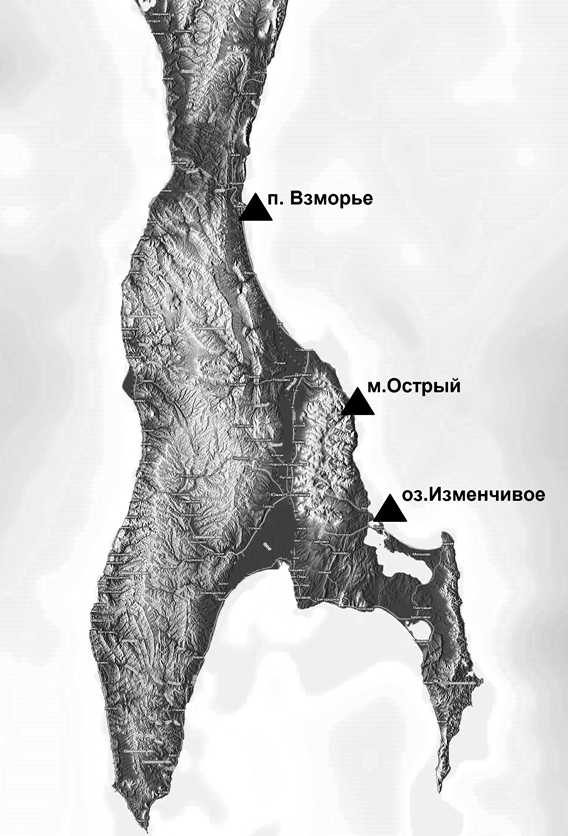
\includegraphics [width=0.5\linewidth] {mapAll.png}
  \caption{Места проведения натурных наблюдений в южной части о. Сахалин}
  \label{img:mapAll}
\end{figure}
\FloatBarrier

В настоящей работе приведены экспериментальные данные, полученные на открытых акваториях или бухтах в районе пос. Взморье, мыса Острый, устья озера Изменчивое острова Сахалин (рис. \ref{img:mapAll}).

В 2007 году в районе пос. Взморье для изучения ветрового волнения в прибрежной зоне и особенностей гидродинамических условий на взморье в летне-осенний период, способствующих абразии, был организован натурный эксперимент, который включал постановку 18 регистраторов придонного давления (АРВ-К12). Донные станции были установлены на различных глубинах – одна группа приборов располагалась ближе к берегу, на глубинах от 5 до 7 м, вторая мористее, на глубинах 10-15 м (рис. \ref{img:mapVzmorie}). Датчики были установлены 14 июля, а подняты 16 октября 2007 года. Значительная часть приборов оказалась замыта, поэтому поднять удалось только пять измерителей. С учетом этого в 2009 году датчики устанавливались на большем расстоянии от берега (1.6-1.8 км) двумя парами – на глубинах 9-10 и 14-15 м, период измерений был с 20 июля по 29 сентября 2009 года.

Натурные наблюдения в районе оз. Изменчивое  (рис. \ref{img:mapIzmenchivoe}) проводились в период с 2 июля по 3 октября 2007 года. Здесь было задействовано 3 регистратора, которые установили на глубинах 12-15 метров в 400 м, 700 м и 900 м от берега.

Аналогичный натурный эксперимент с использованием тех же датчиков проводился в период с 14 июля по 4 августа 2006 года, в районе м. Острый (рис. \ref{img:mapOstry}). В этом эксперименте было установлено 16 регистраторов на глубинах от 7 до 30 метров в двухкилометровой прибрежной зоне, поднять не удалось лишь два из них.

\begin{figure}[h]
\center
\begin{minipage}[h]{0.35\linewidth}
  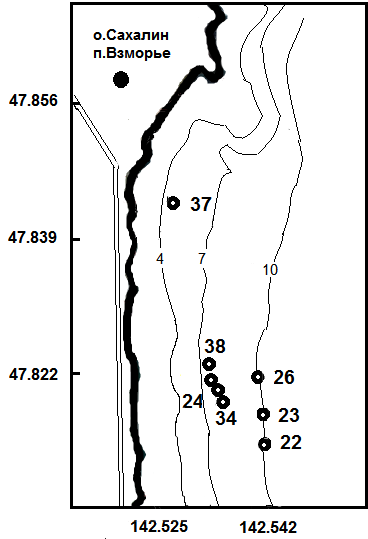
\includegraphics [width=1\linewidth] {mapVzmorie.png}
  \caption{Схема постановки приборов в районе п. Взморье (470 50’ с.ш., 1420 31’ в.д.),}
  \label{img:mapVzmorie}
\end{minipage}
\hfill
\begin{minipage}[h]{0.55\linewidth}
  \center
  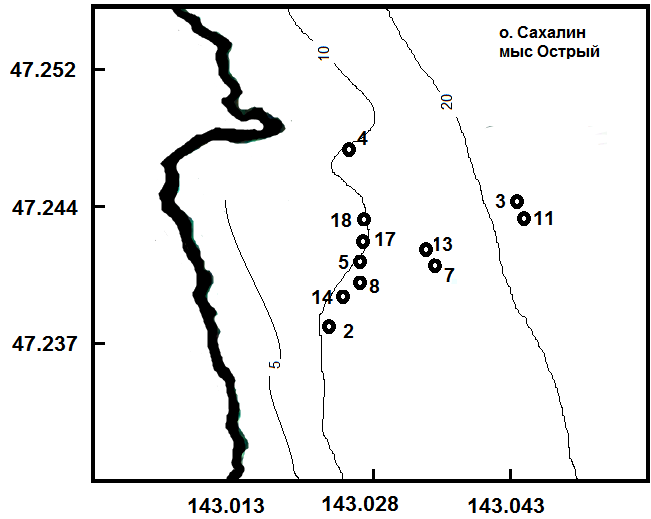
\includegraphics [width=1\linewidth] {mapOstry.png}
  \caption{схема постановки в районе м.Острый (470 14’ с.ш., 1430 1’ в.д.)}
  \label{img:mapOstry}
\end{minipage}
\end{figure}
\FloatBarrier

\begin{figure} [ht]
  \center
  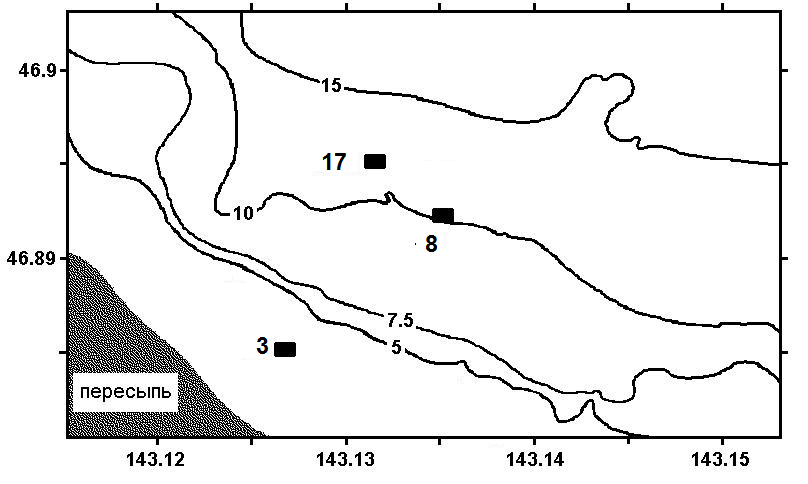
\includegraphics [width=0.9\linewidth] {mapIzmenchivoe.png}
  \caption{Схема постановки в районе оз. Изменчивое (460 9’ c.ш., 1430 13’ в.д.)}
  \label{img:mapIzmenchivoe}
\end{figure}
\FloatBarrier

\section{Определение колебаний уровня моря по данным пульсаций давления на дне}

Датчик придонного давления регистрирует колебания давления, которые в общем случае не совпадают с колебаниями уровня моря. Как известно, поверхностные волны затухают с глубиной, поэтому если использовать только гидростатические соотношения, то донный датчик давления будет занижать амплитуду волн. Эта проблема специально изучалась в различных работах . В рамках линейной потенциальной теории можно получить выражение для спектрального коэффициента ослабления поверхностных волн при измерениях в толще воды, что подробно описано в разделе \ref{linTheory} Главы 1.

 Показанное в этом разделе соотношение \eqref{eq:relationSpectrs} определяет связь спектральных компонент давления (при условии пересчета его в смещение поверхности при использовании гидростатического соотношения) и смещения водной поверхности в Фурье-спектрах волновых полей.

\begin{figure} [ht]
  \center
  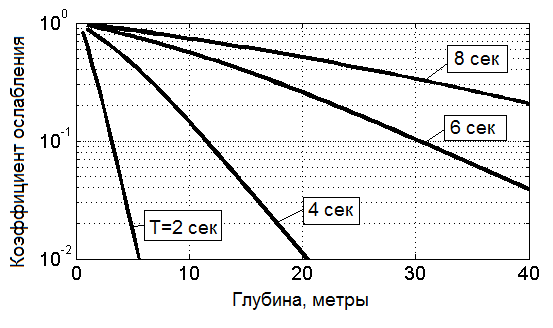
\includegraphics [width=0.9\linewidth] {coeffAttenNature.png}
  \caption{Затухание волн различного периода на различных глубинах}
  \label{img:coeffAttenNature}
\end{figure}
\FloatBarrier

Рассчитанное с помощью \eqref{eq:coeffAtten_W} оно представлено на рис. \ref{img:coeffAttenNature} для интересующего нас диапазона глубин постановки приборов  и периодов волн. Как видно, негидростатические эффекты в поле ветровых волн являются принципиальными и могут кардинально влиять на оценки высот волн.

Точность используемого датчика составляет 0.06\%, то есть при  ослаблении сигнала, более чем в 0,0006 раз шум датчика начинает маскировать реальный сигнал. Это надо учитывать при коррекции сигнала, чтобы не усилить шум прибора, который существенно более высокочастотный, чем ветровое волнение. Поэтому имеет смысл вводить поправочный коэффициент частот ниже 0,25 Гц при постановке датчика на глубину более 40 м. В нашем случае глубины постановки составляют менее 30 метров, поэтому ограничения на поправки становятся более слабые.

\begin{figure} [ht]
  \center
  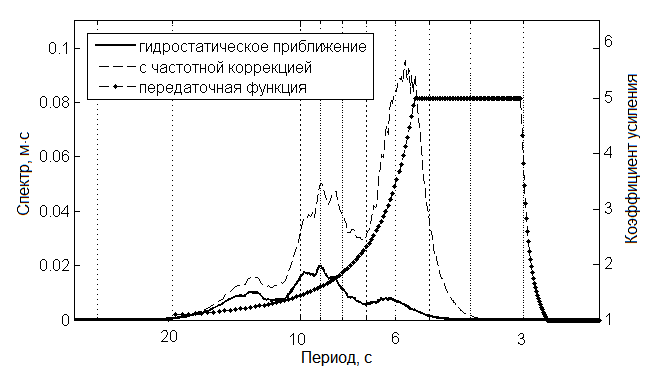
\includegraphics [width=1\linewidth] {spectrCorrect.png}
  \caption{Пример передаточной функции для глубины 16 метров и усредненные спектры рассчитанного  уровня моря по формуле (1) и в гидростатическом приближении}
  \label{img:spectrCorrect}
\end{figure}
\FloatBarrier

На рис. \ref{img:spectrCorrect} представлены амплитудные спектры ветрового волнения и используемая передаточная функция, рассчитанная для этой записи. Поскольку передаточная функция экспоненциально нарастает в области высоких частот (малых периодов), и шум здесь значительно усиливается, то в соответствие с рекомендациями \cite{tucker_2003} ограничили значения передаточной функции величиной 5 и обрезали спектр на частоте 0.33 Гц.

\begin{figure} [ht]
  \center
  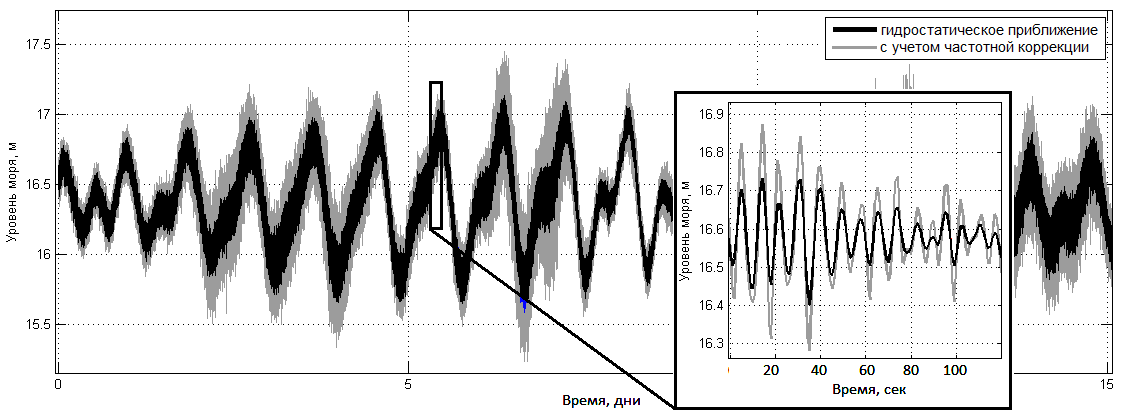
\includegraphics [width=1\linewidth] {waveCorrect_Izmenchivoe.png}
  \caption{Отличие в форме рассчитанных колебаний уровня моря при использовании гидростатической формулы (жирная линия) и с помощью частотной коррекции (тонкая линия). Глубина постановки датчика 16 метров в районе м. Острый}
  \label{img:waveCorrect}
\end{figure}
\FloatBarrier

В результате введенной частотной коррекции поправка в определении смещения уровня воды оказалась существенной, например, для датчика расположенного в районе мыса Острый на глубине 16 метров, высота волны увеличилась примерно вдвое по сравнению с гидростатическим значением (рис. \ref{img:waveCorrect}). Видно, что реальное поверхностное волнение будет существенно отличаться от измеренных флуктуаций давления датчиком придонного давления установленного на глубине более 15 метров и волн с периодами от 1 до 11 с, то есть ветровых волн и зыби. Отметим также, что период и фаза колебаний уровня моря, как видим из рис. \ref{img:waveCorrect}, не меняется при использовании частотной коррекции, а меняется только амплитуда волн.

\begin{figure} [ht]
  \center
  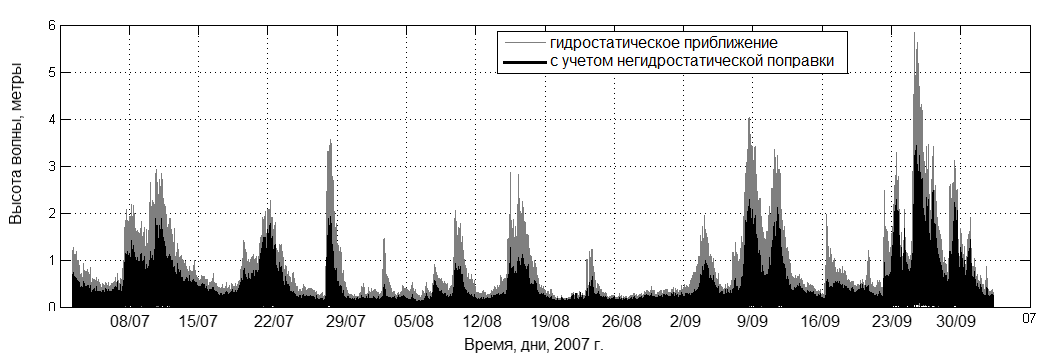
\includegraphics [width=1\linewidth] {heightsCorrect.png}
  \caption{Высоты волн, рассчитанные с учетом негидростатической поправки (черная линия) и без ее учета (серая линия) на озере Изменчивое в 2007 году.}
  \label{img:heightsCorrect}
\end{figure}
\FloatBarrier

На рис. \ref{img:heightsCorrect} представлены рассчитанные высоты волн в районе озера Изменчивое за весь период измерений в 2007 году. Как видим, частотная поправка является принципиальной и разница в значениях высот волн по сравнению с гидростатической оценкой достигает двух раз.

Поскольку использовалась линейная теория для расчета колебаний уровня воды по данным придонного давления, мы специально оценили крутизну волны ka, где а - амплитуда волны. На рис. \ref{img:stepnessNature} представлена рассчитанная крутизна волн по данным, полученным на м. Острый в 2006 году. Как и следовало ожидать, негидростатическое приближение увеличивает крутизну волн. Как видим, в спокойные периоды крутизны волн не превышают 0.05, что соответствует линейным волнам \cite{Holth_2007}. Количество таких волн для оцениваемого периода в 20 суток составило 98.7\%, так что в среднем использование линейной теории можно считать правомерным. Разумеется, более точные оценки применимости линейной теории должны быть получены из нелинейной теории, что пока не сделано. Поэтому вслед \cite{Huang_Tsai_2008} мы будем использовать линейную теорию для коррекции рассчитанных колебаний уровня моря.

\begin{figure} [ht]
  \center
  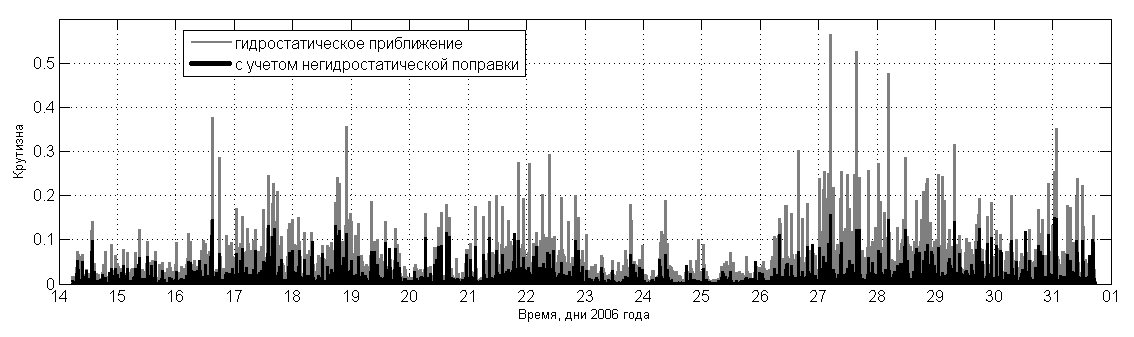
\includegraphics [width=1\linewidth] {stepnessNature.png}
  \caption{Оценка крутизны волн при использовании гидростатической формулы (серая линия) и с учетом негидростатической поправки (черная линия) по данным полученным вблизи м. Острый в 2006 году.}
  \label{img:stepnessNature}
\end{figure}
\FloatBarrier

В соответствие с описанной методикой, процедуру предварительной коррекции прошли все анализируемые в работе записи. Был разработан программный комплекс, состоящий из набора вычислительных программ реализованных в С++, и скриптов на языке Matlab, для отображения и анализа результатов вычислений, особенно вычислений высот и периодов волн. Ниже будут проанализированы высоты и периоды волн по данным инструментальных наблюдений.

\subsubsection{Дискретизация ветрового волнения}
Спектр колебаний поверхности моря может быть достаточно сложным, что является следствием влияния на него различных океанологических процессов. Так, например, цунами имеют характерные периоды от 2 мин. до 2 часов. И для их изучения в соответствии с теоремой Котельникова \cite{kotel} достаточной оказывается дискретность измерений 1 мин. Но поскольку спектр колебаний уровня моря содержит и более короткие колебания, то во избежание алиасинга при регистрации, например, волн цунами с такой дискретностью, ранее применялись цифровые фильтры низких частот, «обрезавшие» ветровое волнение и зыбь. В настоящее время в большинстве гидрофизических приборов, предназначенных для регистрации колебаний уровня (давления), используется дискретность 1 с, которой вполне достаточно для записи ветровых волн с периодами от 3 с и длиннее \cite{kovalev_2011}, и которые, как показывают результаты наших наблюдений в прибрежной зоне Тихого океана, присутствуют в спектрах волнения. Тем не менее, ряд авторов \cite{kabat_2007, abrosim} показали в их записях наличие волн и с меньшими периодами. Это обстоятельство, в принципе, может приводить к возникновению алиасинга, искажающего спектр длиннопериодных волн.

Для выяснения вопроса о достоверности измерений в подобных условиях 18 мая 2011 г. вс. Охотское был проведен специальный эксперимент. Два различных датчика - кабельный датчик гидростатического давления и струнный датчик, регистрирующий непосредственно
колебания морской поверхности, устанавливались в одной точке (рис. \ref{img:discr_2}), и велась синхронная запись колебаний уровня моря с регистрацией на ноутбук.

\begin{figure} [ht]
  \center
  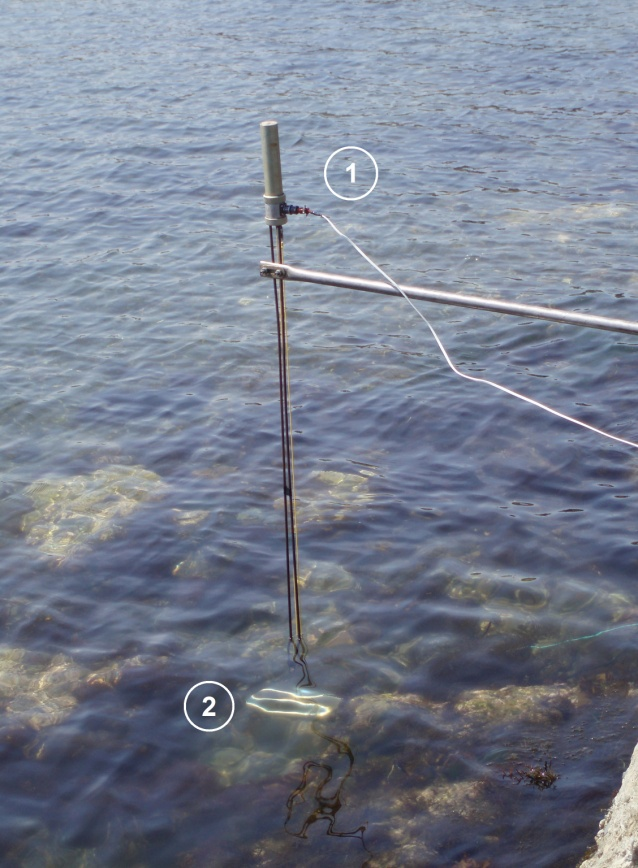
\includegraphics [width=0.5\linewidth] {discr_2.jpeg}
  \caption{Установка струнного датчика волнения (1) и гидростатического давления (2)}
  \label{img:discr_2}
\end{figure}
\FloatBarrier



В результате были получены цифровые записи ветрового волнения с дискретностью 6 отсчетов в секунду, приведенные на рис. \ref{img:discr_3}. На записи струнного датчика присутствуют колебания с периодами около 0.8 с, обусловленные короткопериодными капиллярными волнами. Во временном ходе гидростатического датчика, несмотря на малую глубину его постановки - около 45 см, такие колебания отсутствуют, что связано с сильным затуханием этих волн с глубиной.

\begin{figure} [ht]
  \center
  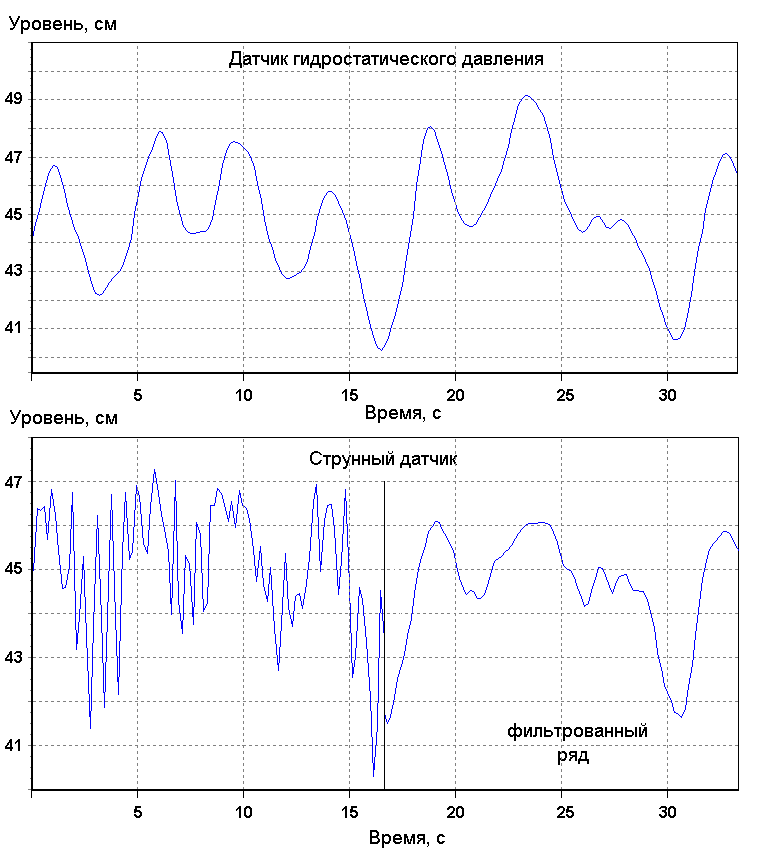
\includegraphics [width=0.7\linewidth] {discr_3.png}
  \caption{Временной ход колебаний уровня моря, записанный синхронно датчиком гидростатического давления и струнным (емкостным) датчиком}
  \label{img:discr_3}
\end{figure}
\FloatBarrier

Для ветрового волнения записи обоих датчиков имеют схожий вид, что также подтвердила выполненная нами низкочастотная фильтрация данных струнного датчика простым «треугольным» фильтром.

Для полученных рядов наблюдения были рассчитаны энергетические спектры, приведенные на рис. \ref{img:discr_4}. Видно, также как и из временного хода колебаний уровня, что в спектре струнного датчика, в отличие от гидростатического, присутствует значимый подъем энергии на периодах от 1.3 до 0.3 с, связанный с короткопериодными капиллярными волнами.

\begin{figure} [ht]
  \center
  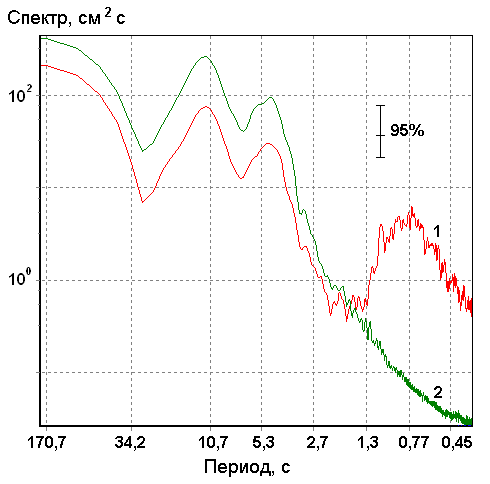
\includegraphics [width=0.7\linewidth] {discr_4.png}
  \caption{Энергетические спектры колебаний уровня моря. 1 -- струнный датчик, 2 -- датчик гидростатического давления}
  \label{img:discr_4}
\end{figure}
\FloatBarrier


Поскольку спектр датчика гидростатического давления на периодах короче 2.7 с не имеет сколько-нибудь значимых пиков и спадает в среднем около 8 дБ на октаву, что примерно соответствует фильтрации исходного процесса однозвенным низкочастотным фильтром, то для него можно говорить о естественном ограничении спектра волнения и возможности дискретизации физического аналогового процесса волнения с дискретностью 1 с без наличия эффекта алиасинга.

В спектрах струнного датчика содержатся значимые составляющие с периодами меньше 1 секунды. Для ограничения их спектра была проверена возможность создания простого, интегрирующего по времени измерения фильтра, который может быть просто организован в цифровых схемах измерения.

Такая фильтрация с временным окном 0.5 с использовалась для сглаживания данных струнного датчика с частотным выходным сигналом и показала хорошие результаты (рис. \ref{img:discr_3}). При этом условии, т. е. при установке в его схеме интегрирующего счетчика, он также может использоваться для регистрации колебаний уровня моря с дискретностью 1 с.

\section{Спектральные характеристики}

\subsection{Анализ данных полученных м.Свободный в 2011 году}

В соответствии с описанной выше методикой были скорректированы данные, полученные в результате эксперимента в районе  мыса Свободный с октября 2011 года по май 2012 года.  График уровня моря, рассчитанный по этим данным с учетом гидростатической поправки, представлен на рис. \ref{img:svobodny_1}.


\begin{figure} [ht]
  \center
  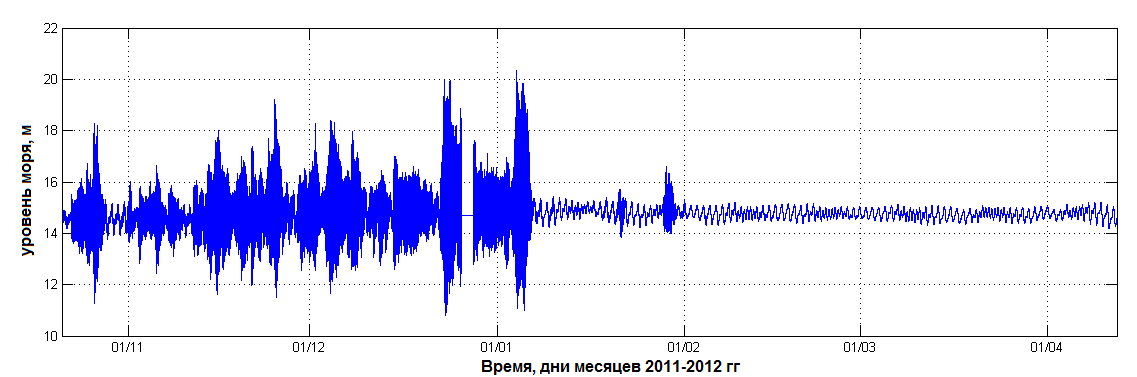
\includegraphics [width=\linewidth] {svobodny_1.png}
  \caption{График уровня моря, рассчитанные с учетом гидростатической поправки по данным натурных наблюдений в районе м. Свободный 2011-2012 гг.}
  \label{img:svobodny_1}
\end{figure}
\FloatBarrier

Предварительный анализ колебаний обнаруживает множество сильных штормов в период наблюдений с ноября по декабрь 2011 года. Наиболее сильный шторм отмечается в конце декабря - начале января с амплитудой ветрового волнения до 9 метров. Ниже представлен график значительных высот волн, рассчитанный по этим колебаниям, по которому также можно отметить высокую штормовую активность и связанные с этим относительно большие значительные высоты волн, что в целом является характерным для данного региона.

\begin{figure} [ht]
  \center
  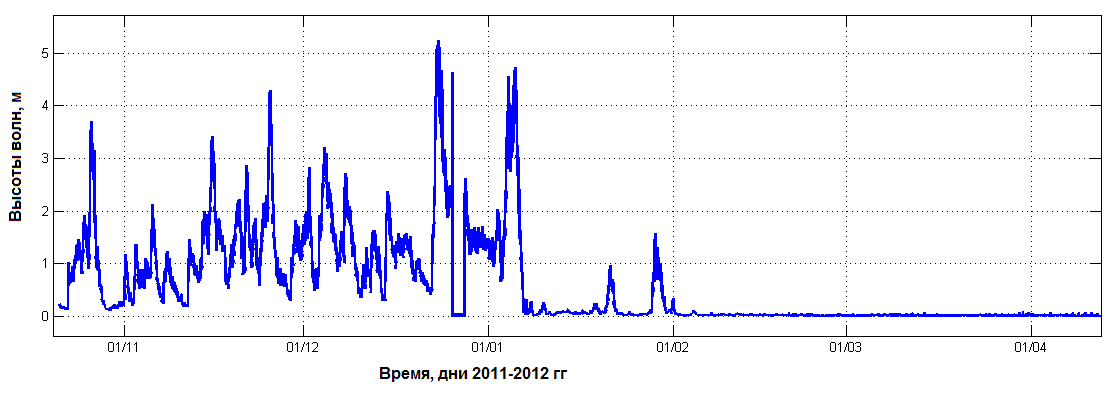
\includegraphics [width=\linewidth] {svobodny_2.png}
  \caption{Значительные высоты волн, рассчитанные с учетом гидростатической поправки по инструментальным наблюдениям в районе м. Свободный 2011-2012 гг.}
  \label{img:svobodny_2}
\end{figure}
\FloatBarrier


Одной из интересных отличительных особенностей полученных записей является то, что на них присутствуют участки, когда датчик регистрировал волнение моря, покрытого льдом [15]. Таким образом, у нас есть возможность отследить изменение различных характеристик (спектральных, статистических) волнения не только во время изменения режима волнения, но и во время установления ледового покрова.
Для оценки изменения спектральных характеристик во времени, по всей записи был построен текущий спектр, представленный на рис. \ref{img:svobodny_3} и рис. \ref{img:svobodny_4}.

\begin{figure} [ht]
  \center
  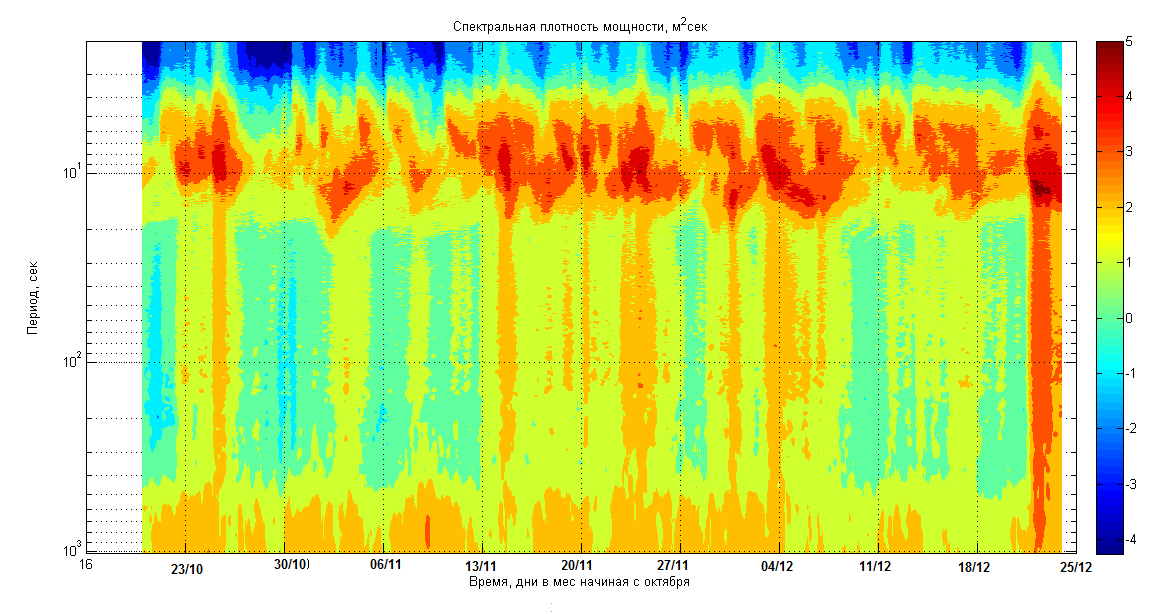
\includegraphics [width=0.8\linewidth] {svobodny_3.png}
  \caption{Текущий спектр, рассчитанный для участка записи с 23.10.2011 по 25.12.2011, по данным, полученным вблизи м. Свободный}
  \label{img:svobodny_3}
\end{figure}
\FloatBarrier

\begin{figure} [ht]
  \center
  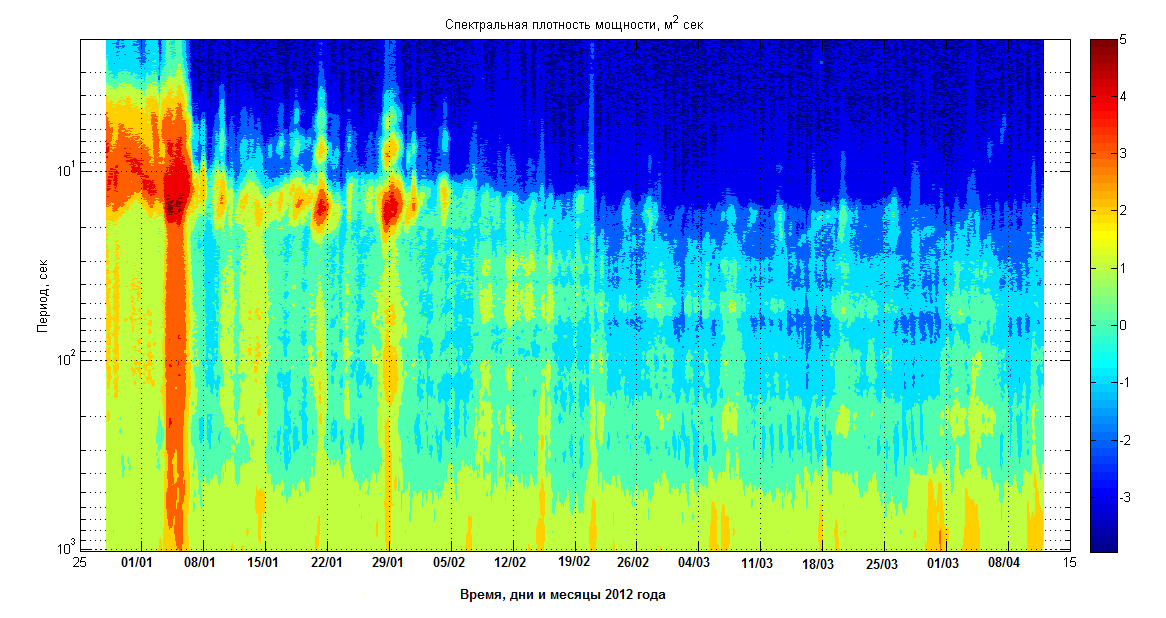
\includegraphics [width=0.8\linewidth] {svobodny_4.png}
  \caption{Текущий спектр, рассчитанный для участка записи с 01.01.2012 по 10.04.2012, по данным, полученным вблизи м. Свободный}
  \label{img:svobodny_4}
\end{figure}
\FloatBarrier

По рис.\ref{img:svobodny_3} и рис.\ref{img:svobodny_4} видно, что периоды наиболее сильных спектральных пиков приходятся на диапазон волнения от 5 до 12 секунд. На записи удалось зарегистрировать два наиболее сильных шторма: 24 декабря 2011 года и 5 января 2012 года. Во время этих событий заметно существенное усиление не только ветровых волн и волн зыби, но и энергии в области инфрагравитационных волн. Стоит особо отметить резкое изменение спектра волн после этих штормов. 7 января энергия в области ветровых волн, высокочастотной и среднечастотной зыби резко падает, что очевидно связано с влиянием ледового покрова моря на волнение. Вероятно, лед был подогнан к берегу сильными штормами. 22 и 29 января на спектре отмечаются интересные усиления в области зыби с периодами 15-18 секунд, зародившейся вероятно еще в Тихом океане, поскольку такие низкие периоды зыби не характерны для зыби, образующейся в Охотском море.

Характер распределений  иллюстрируется вычисленными коэффициентами асимметрии и эксцесса (рис.\ref{img:svobodny_7} и рис.\ref{img:svobodny_8}):

\begin{equation}\label{eq:assimEx}
  Sk=\frac{1}{N\sigma^3}\sum\limits_{i=1}^N[z_i-<z>]^3, Ku=\frac{1}{N\sigma^4}\sum\limits_{i=1}^N[z_i-<z>]^4
\end{equation}

\begin{figure} [h]
  \center
  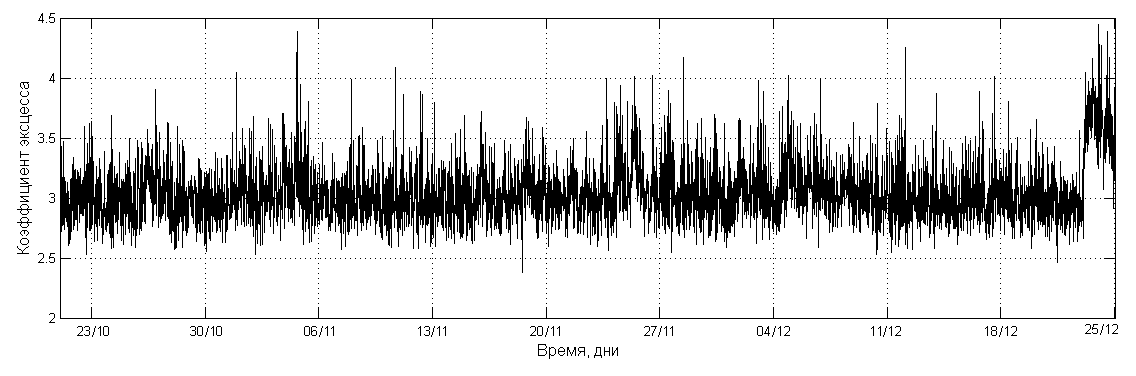
\includegraphics [width=\linewidth] {svobodny_7.png}
  \caption{Временная изменчивость коэффициента эксцесса в период с 21 октября  по 27 декабря 2012 в районе м.Свободный.}
  \label{img:svobodny_7}
\end{figure}
\FloatBarrier



\begin{figure} [h]
  \center
  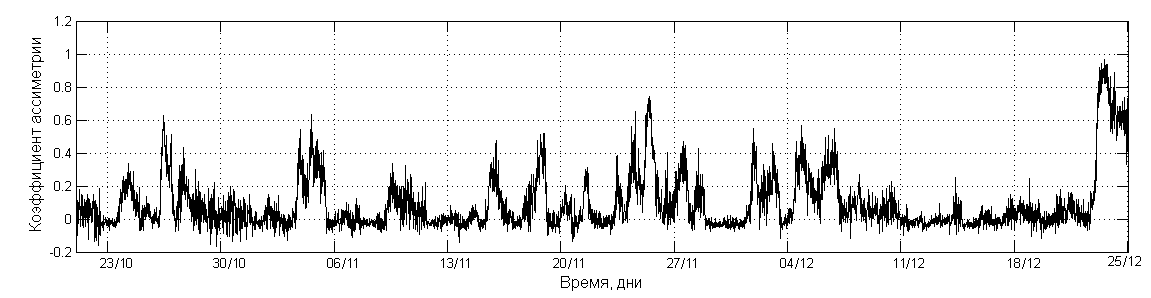
\includegraphics [width=\linewidth] {svobodny_8.png}
  \caption{Временная изменчивость коэффициента ассиметрии в период с 21 октября  по 27 декабря 2012 в районе м.Свободный.}
  \label{img:svobodny_8}
\end{figure}
\FloatBarrier


Графики коэффициентов ассиметрии и эксцесса, представленные на рис.\ref{img:svobodny_7} и рис.\ref{img:svobodny_8}, обнаруживают сильную изменчивость в течение 70 суток, однако средние значения этих коэффициентов ($<Sk>$ = 0.0920, $<Ku>$ = 3.0427) достаточно мало отличаются от «гауссовых» значений ($Sk$ = 0 и $Ku$ = 3), так что в целом ветровое волнение является почти гауссовым процессом. Отчетливо видно, что во время штормов функция распределения смещения поверхности становится асимметричной (положительный третий момент), следовательно число больших гребней превышает число больших "ям" и волновой процесс становится более нелинейным. Также чуть большее значение коэффициента эксцесса (по сравнению с гауссовым) свидетельствует о большей вероятности появления аномально больших волн, чем это предсказывает распределение Рэлея.

\subsection{Анализ данных полученных в районе п.Взморье}

Для исследования гидродинамических процессов в прибрежной зоне моря, обусловленных трансформацией ветрового волнения на мелководье и формированием длинных инфрагравитационных волн, был организован натурный эксперимент, который включал постановку группы измерителей придонного гидростатического давления. Приборы были выставлены плотной группой в районе интенсивного размыва автомобильной дороги (106-108 километр), несколько датчиков были расположены севернее, вблизи пос.Взморье. Схема постановки приборов представлена на рис.4.1.
Ближе всего к берегу находилась станция 36 (глубина около 6 м), единственная из серии выставленных в ближней зоне, которую удалось найти и поднять, но она находилась несколько в стороне от основной группы регистраторов. Самым удаленным был датчик 26 (глубина около 15 м),  вместе с ним приборы 29 и 24 образовывали приблизительно прямую линию, ориентированную по нормали к берегу. Анализу записей на этих приборах уделялось основное внимание. Расстояние между станциями 26 и 29 составляло 580 м, между 29 и 24 - 130 м.


\begin{figure} [ht]
  \center
  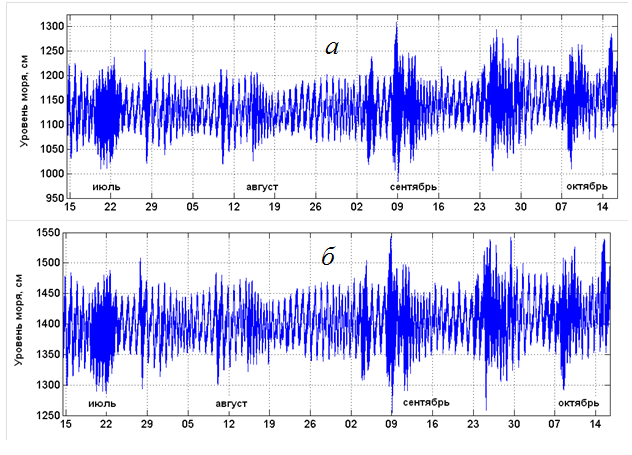
\includegraphics [width=\linewidth] {vzmorie_1.png}
  \caption{Измеренные значения придонного гидростатического давления на датчиках 24 (а) и 26 (б), пересчитанные в см водного столба}
  \label{img:vzmorie_1}
\end{figure}
\FloatBarrier

На рис.\ref{img:vzmorie_1} представлены графики придонного гидростатического давления на более близкой к берегу станции 24 и самом удаленном датчике 26. В большинстве случаев в них преобладают приливные колебания уровня моря, что, очевидно, отвечало спокойным погодным условиям и сравнительно слабому волнению. Хотя большинство датчиков располагалось на глубинах 10 м и более, волны зыби достаточно хорошо прописывались на донных регистраторах даже в сравнительно спокойную погоду, но были особенно заметны, когда волнение резко усиливалось, и эти штормовые ситуации на рис.5. проявляются как темные пятна. Один серьезный шторм отмечен в середине июля, еще четыре осенью, в сентябре – октябре. Наибольший размах колебаний наблюдался при сильном шторме в начале сентября – на более близкой к берегу станции 24 он достигал 3 м, на более удаленной 26 – около 2.5 м. Нужно отметить, что изучаемый район прикрыт от подхода волн северо-восточного и близких к нему румбов полуостровом Терпения. Нужно отметить, что именно это направление является наиболее опасным, так как в тыловой части циклонов обычно наблюдаются сильные и устойчивые северо-восточные и северные ветра, для которых имеется достаточная длина разгона. Для юго-восточных ветров, типичных для переднего фронта, она ограничена Южными Курильскими островами. Для сравнения, при шторме 25-26 сентября в районе оз.Изменчивое, расположенном примерно в 100 км к югу от пос.Взморье, высота ветровых волн достигала 4.5 м [Shevchenko et al, 2009], что примерно вдвое больше, чем на станции 24.

Расчет характеристик ветрового волнения на поверхности моря осуществлялся для каждого последовательного 15-минутного интервала при помощи программы, предоставленной нам д.ф.м.н. И.М.Кабатченко (ГОИН) \cite{kabat_2007}. Рассчитывался спектр волнения, значимая высота волны и период главного спектрального максимума. Рассчитанные спектры сводились в таблицу, по которой производилось построение диаграммы текущего спектра. По вертикальной оси диаграммы откладывались частоты (периоды) колебаний, по горизонтальной – время. На рис.\ref{img:vzmorie_2}, рис.\ref{img:vzmorie_3} представлены спектрально-временные диаграммы для расположенных на различном расстоянии от берега станций 24 и 26 за относительно спокойный период – август 2007 года.

\begin{figure} [ht]
  \center
  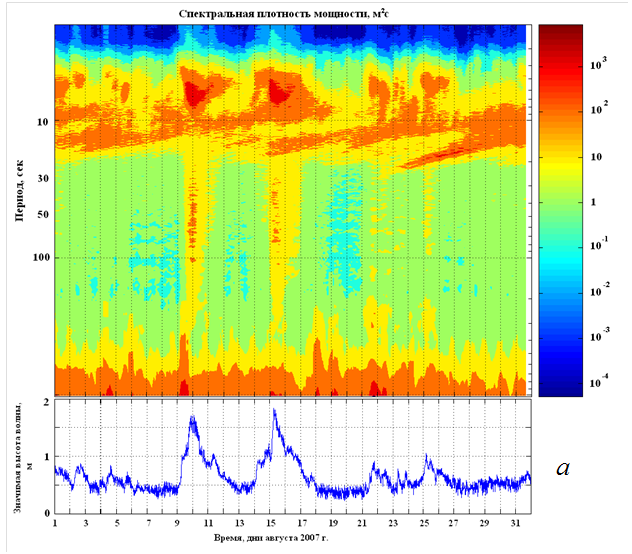
\includegraphics [width=0.8\linewidth] {vzmorie_2.png}
  \caption{Спектрально-временная диаграмма волнения на станциях 24 в августе 2007 года, расчет спектров выполнен по последовательным отрезкам продолжительностью 15 мин. Внизу приведены графики вариаций значимой высоты волны, рассчитанной за эти же промежутки времени.}
  \label{img:vzmorie_2}
\end{figure}
\FloatBarrier

\begin{figure} [ht]
  \center
  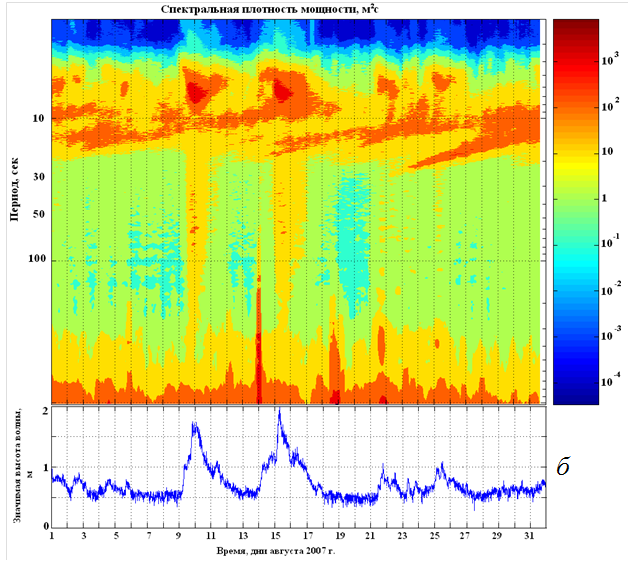
\includegraphics [width=0.8\linewidth] {vzmorie_3.png}
  \caption{Спектрально-временная диаграмма волнения на станциях  26 в августе 2007 года, расчет спектров выполнен по последовательным отрезкам продолжительностью 15 мин. Внизу приведены графики вариаций значимой высоты волны, рассчитанной за эти же промежутки времени.}
  \label{img:vzmorie_3}
\end{figure}
\FloatBarrier

В записях волнения в течение всего периода наблюдений явно преобладали волны зыби с периодами 7-9 сек, на диаграмме они проявляются в виде довольно широкой, хорошо выраженной полосы. Особенно мощно выделялся пик на периоде 8 сек даже при сравнительно слабых штормах 8 и  15 августа (значимая высота волны достигала 2 м), причем это проявилось на всех станциях. В некоторых случаях можно отметить, помимо указанной полосы, усиление более низкочастотных колебаний, с периодами 10-15 секунд, причем изменение периода энергетического максимума колебаний происходило равномерно, каждый раз наиболее низкочастотные волны проявлялись раньше, и период во времени уменьшался (полоса имеет характерный наклон).

В некоторых ситуациях этот низкочастотный пик является основным, что характерно для спокойных погодных условий. Наиболее низкочастотные волны были обнаружены при анализе волновых процессов 23-26 августа. В этот период отмечены волны зыби с периодом около 20 сек, но их высота была сравнительно небольшой, около полуметра. Наиболее вероятно, это связано с проникновением океанской зыби в Охотское море – в изучаемом районе волны с такими пространственно-временными масштабами вряд ли могли образоваться.

Другой примечательной особенностью, отмеченной при анализе спектрально-временных диаграмм, явилось резкое (примерно на два порядка) возрастание энергии колебаний в диапазоне инфрагравитационных волн (периоды от 20-200 сек) при штормовых ситуациях. При этом в указанном диапазоне не наблюдается четких, хорошо выраженных максимумов как на удаленной станции 26, так и на более близкой к берегу станции 24. Когерентность в диапазоне инрагравитационных волн невелика, поэтому анализировать фазовые спектры между данными станциями не имеет смысла. Возможно, расстояние между приборами было слишком большим в данном случае для подобных расчетов.

\subsection{Анализ данных полученных в районе м.Острый}

Спектральный анализ волнения производился с помощью алгоритма Уэлча. Данный метод является одним из наиболее популярных методов спектральной оценки, он дает эффективное усреднение дискретного спектра и устранение изрезанности с уменьшением дисперсии оценки.  На (рис. \ref{img:ostry_1}) представлена оценка амплитудного спектра, рассчитанного по данным придонного датчика давления, находящегося подо льдом.


\begin{figure} [ht]
  \center
  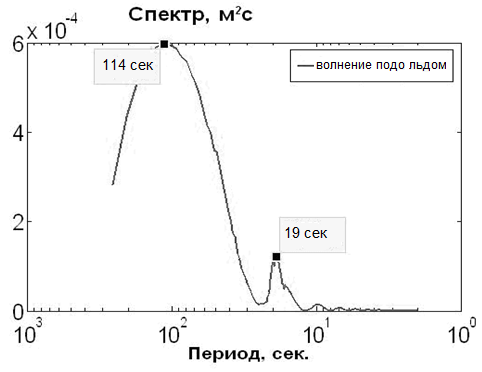
\includegraphics [width=0.5\linewidth] {ostry_1.png}
  \caption{Оценка амплитудного спектра волнения, вычисленного по данным датчика придонного  давления, находящегося подо льдом.}
  \label{img:ostry_1}
\end{figure}
\FloatBarrier

На этом спектре видно полное отсутствие энергии волн с периодами меньше чем 16 секунд. Лед защищает поверхность воды от воздействия ветра, следовательно, невозможно образование ветровых волн, период которых обычно составляет от 4 до 6 секунд. Поэтому на спектре обнаруживается лишь длинноволновая зыбь с периодом около 18 секунд. Эта зыбь пришла сюда по-видимому из Тихого океана, но и она потеряла большую часть энергии из-за ледового покрова, видно что ее энергия существенно ниже энергии инфрагравитационных волн.

\begin{figure} [ht]
  \center
  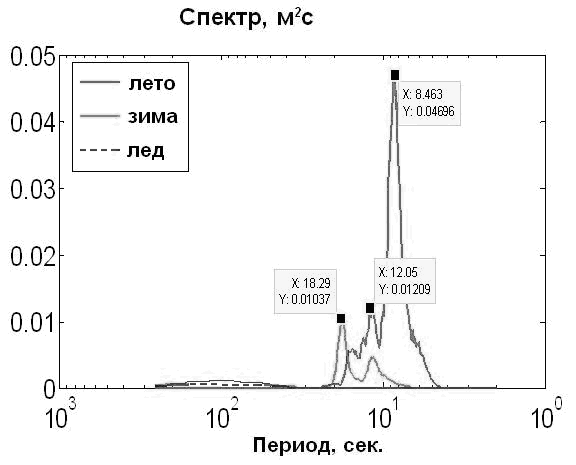
\includegraphics [width=0.5\linewidth] {ostry_2.png}
  \caption{Оценка амплитудного спектра волнения, вычисленного по данным датчика придонного  давления}
  \label{img:ostry_2}
\end{figure}
\FloatBarrier
На (рис.\ref{img:ostry_2}) представлены спектры для различных условий: при наличии ледяного покрова в спокойную погоду, при зимнем шторме, при летнем шторме. Хорошо видно, что энергия инфрагравитационных волн (с периодами от 30 секунд до 30 минут) практически не изменилась. При летнем шторме заметно усиление зыби с периодами 8-9 секунд. Так же виден небольшой пик в области ветровых волн с периодом 5 секунд. Тогда как подобных пиков при зимнем шторме не зарегистрировано, что, скорее всего, связано с тем, что шуга и мелкие куски льда, отколовшиеся от угнанного штормом ледяного покрова, гасят короткие ветровые колебания. Также в записи зимнего шторма четко виден спектральный пик в области 18 секунд, что связано, видимо с проявлением длинноволновой зыби, зародившейся в Тихом океане.

\subsubsection{Спектрально-временной анализ}


\begin{figure} [ht]
  \center
  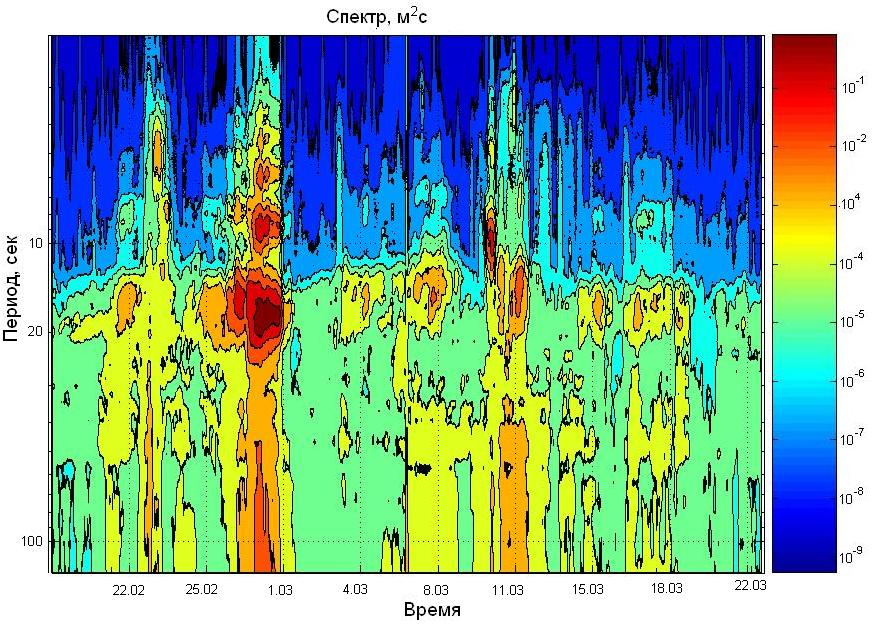
\includegraphics [width=1\linewidth] {ostry_3.jpeg}
  \caption{Спектрограмма, рассчитанная по записи, полученной в районе м. Острый  за период 18.02.2007 – 23.03.2007}
  \label{img:ostry_3}
\end{figure}
\FloatBarrier

На рисунке выше представлена спектрограмма колебаний  с 21 степенью свободы, которые характеризуют степень доверия к спектральной оценке.  Начало записи 18.02.2007 соответствовало покрытому льдом морю. Поэтому на спектрограмме видно, что волны с периодами меньше 16 секунд имеют низкий уровень энергии 10-8 м2с, а далее до 22.02.2007 идет нарастание энергии и 23.02.2007 заметен довольно мощный пик в области ветровых волн с энергией 10-3 м2с, который свидетельствует о небольшом шторме. После прекращения шторма 24.02.2007 энергия в области ветровых волн спадает до 10-7 м2с, так же виден более высокий уровень энергии в области среднепериодной зыби 10-6 м2с.  26.02.2007 виден мощный шторм, который пришел видимо со стороны океана, потому что зарегистрирована большая энергия в области океанической длинноволновой зыби (зыбь с периодами 18-20 секунд). Шторм резко стихает 1.03.2007 и уровень энергии среднечастотной зыби и ветровых волн снова спадает до 10-8  м2с, это обусловлено, скорее всего с тем, что сильный ветер, связанный со штормом, пригнал лед и шугу в этот район. После 4.03.2007 уровень энергии зыби и ветровых волн повышается, что, очевидно, связано с отходом и таянием льда. Так же заметен резкий скачок энергии на значении периода в 12 секунд, это можно объяснить геометрией бухты, в которой стоял датчик

\subsubsection{Групповая структура волнения}

Групповая структура волн, проявляющаяся в чередовании цугов высоких и низких волн, является неотъемлемой чертой как штормовых волн, так и волн зыби, а ее изменчивость во времени и пространстве вызывает колебания высших моментов волнового движения (асимметрия, эксцесс и др.), чрезвычайно важных для описания многих динамических процессов в береговой зоне моря. Производимые группами волн инфрагравитационные колебания вместе с самой групповой структурой волн приводят к перемежаемости процессов взвешивания и транспорта осадков, образованию тягуна в портах и гаванях, а также экстремальным нагрузкам на береговые сооружения.

Цуг волн есть ряд возмущений с перерывами между ними.  Одно возмущение называется волновым пакетом.
Для выделения групповой структуры волн различных частотных диапазонов использовались огибающие волны, вычисляющиеся как:
\begin{equation}\label{eq:hilbert}
  H_e(t)=\sqrt{{L[H(t)]}^2+[X{L[H(t)]}]^2},
\end{equation}
где $X$ – преобразование Гильберта, $L$ – оператор линейной фильтрации, оставляющий лишь частоты требуемого диапазона, а $H(t)$ – возвышения свободной поверхности. При использовании частотного диапазона с шириной, большей минимальной частоты $f_{min}$ этого диапазона, проводилась дополнительная фильтрация огибающей, удалявшая частоты большие $f_{min}$. Высота и период групп волн оценивались по флуктуациям огибающей.

Функции спектральной плотности огибающих нерегулярного волнения достаточно широки и имеют множество трудно интерпретируемых особенностей. Поэтому использовались два интегральных параметра, характеризующих относительные высоту и период групп волн: фактор групповитости $GF$ и среднее число волн в группе $NW$. $GF=1.41SHe/Hm$, где $Hm$ – средняя по времени величина огибающей, равная половине средней высоты волн, а $SHe$ – стандартное отклонение огибающей от ее среднего значения. Большие значения $GF$ соответствуют более выраженной групповой структуре, нулевое значение GF свидетельствуют об ее отсутствии. $NW$ равнялось отношению средней частоты огибающей к средней частоте волн. Средняя частота спектра волн ($\bar{f}$) и средняя частота спектра огибающей волн ($\bar{f_e}$) рассчитывались как отношение первого спектрального момента к нулевому. Моменты частотного спектра рассчитывались как
$$
m_i=\int\limits_0^{\infty}f^iS(f)df,
$$
где $S$ – спектральная плотность.

Для более удобной работы с огибающими и исходными колебаниями была разработана программа с графическим пользовательским интерфейсом, в ней были реализованы алгоритмы построения огибающей и фильтрации данных (Подробное описание и руководство к программе смотрите в Приложении).
Чтобы построить огибающую необходим узкополосный сигнал,  поэтому данные фильтровались настраиваясь на зыбь в 12-14 секунд, которая является характерной для этого района. После этого строилась огибающая отфильтрованного ряда.


\begin{figure} [ht]
  \center
  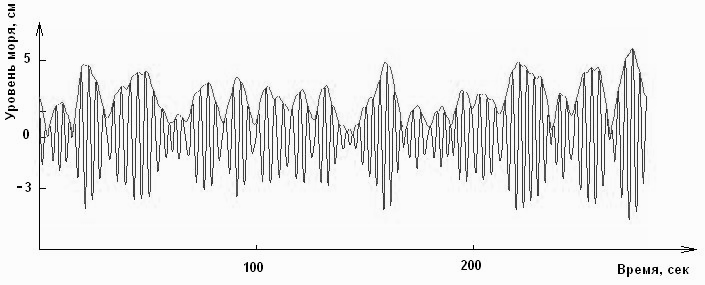
\includegraphics [width=1\linewidth] {ostry_4.png}
  \caption{Пример огибающей волнения, рассчитанной по записи, в районе м. Острый  в марте 2007 года}
  \label{img:ostry_4}
\end{figure}
\FloatBarrier


\begin{figure} [ht]
  \center
  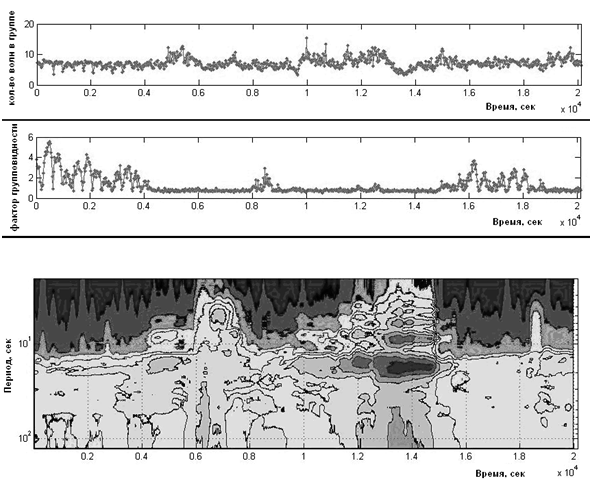
\includegraphics [width=1\linewidth] {ostry_5.png}
  \caption{График зависимости количества волн в группе от времени, по записи}
  \label{img:ostry_5}
\end{figure}
\FloatBarrier

На (рис. \ref{img:ostry_5}) представлена оценка параметров $NW$ и $GF$, хорошо видно, что в начале записи (18.02.2007—22.02.2007) количество волн в группе остается постоянным, в то время когда присутствует ледовый покров, при этом заметны высокие значения фактора групповидности и очень хорошо прослеживается групповая структура волнения в этот момент.  Во время штормов групповая структура прослеживается хуже, разброс количества волн в группе резко увеличивается.

\subsubsection{Основные выводы спектрального анализа натурных наблюдений в районе м.Острый в 2006-2008 году}

Рассматривая полученные результаты обработки данных по эксперименту в районе м.Острый, было сделано несколько основных выводов:
1)	Спектральная оценка записей, соответствующих покрытому льдом морю,  показывает практически полное отсутствие энергии в области ветровых волн, высокочастотной и низкочастотной зыби. Заметна только зыбь, образовавшаяся в Тихом океане,  где нет стабильного ледяного покрова.

2)	Ледовый покров не влияет на энергию в области инфрагравитационных волн.

3)	Штормы в зимний период характеризуются большей энергией в области низкочастотной зыби (период 18-20 сек), чем в области среднечастотной (период 17-12 секунд), высокочастотной (7-11 сек) зыби и ветрового волнения. В летний период при шторме заметно более сильное увеличение ветровых волн и высокочастотной зыби.

4)	В исследуемом районе часто проявляются волны с периодом 12-14 с.,  волны с периодом ниже этой границы, т.е. ветровые и высокочастотная зыбь имеют энергию существенно более низкую. Что связано, возможно, с присутствием мыса Острый, который и задерживает высокочастотное волнение.

5)	На записях соответствующих волнению моря, покрытому льдом, отмечаются высокие значения фактора групповидности (волны хорошо формируют группы) а также среднее количество волн в группе почти не меняется.


\section{Статистические характеристики}
Уже отмечалось во введении, что в регистре \cite{spravWind_2003} приводятся некоторые усредненные статистические характеристики ветрового волнения, такие как повторяемость различных высот и периодов волн, скоростей и направлений ветра, длительности штормов и окон погоды, высоты волн возможные 1 раз в 5, 10, 25, 50, 100 лет.  Эти значения для юго-востока Сахалина рассчитаны по данным визуальных наблюдений со станции Стародубское (47024’ с.ш., 142049’ в.д.), а также по гидродинамической модели WAVEWATCH III, верифицированной по северным точкам, вблизи залива Одопту (580 06’ с.ш., 1430 28’ в.д.). Инструментальные данные, приводимые в настоящей работе, позволяют изучить распределения элементов волн для конкретных пунктов вблизи побережья Сахалин.

\subsection{Распределения высот волн}

В данной работе высота волны рассчитывалась как расстояние от подошвы волны до гребня (т.е. вторичные экстремумы в записи, не пересекающие среднюю волновую линию, не учитываются)\cite{Huang_Tsai_2008}. Для анализа использовано три рассчитанные с учетом негидростатических эффектов записи волн вблизи оз. Изменчивое, семь вблизи п. Взморье, продолжительностью около 3 месяцев, каждая из которых насчитывает около 1 млн. волн и 10 записей вблизи м. Острый продолжительностью 18 дней, каждая из которых содержит 200 тыс. волн. Для учета нестационарности процесса, как это принято в океанологии, запись разбивалась на квазистационарные участки продолжительностью 20 минут, по которым рассчитывался средний уровень и значительная высота волны, (как средняя высота 1/3 самых высоких волн). На рис. \ref{img:heightsAndHs} показан пример временной изменчивости высот волн и значительной высоты волны в течение 2 часов 27 июля 2006 года на датчике вблизи м. Острый.

\begin{figure} [ht]
  \center
  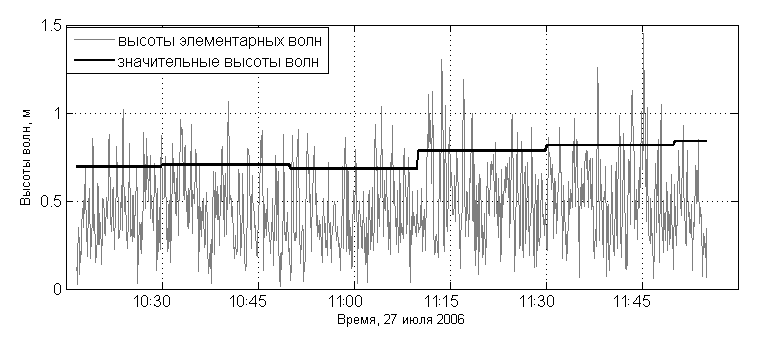
\includegraphics [width=1\linewidth] {heightsAndHs.png}
  \caption{График изменчивости высот волн и значительный высоты волны, по данным полученным 27.07.2006 в районе м.Острый.}
  \label{img:heightsAndHs}
\end{figure}
\FloatBarrier

Как и следовало ожидать, высоты индивидуальных волн в записи могут превышать значительную высоту волны, в частности на рис. \ref{img:heightsAndHs} в два раза, так что такие волны относятся к категории волн - убийц \cite{6_Kurkin_freak} \cite{13_Kharif_2009}. Рис. \ref{img:hs_windSpeed} демонстрирует связь значительной высоты волны со скоростью ветра. К сожалению, мы не располагаем полем ветра в точке измерений и скорость ветра взята из данных наблюдений о фактической погоде, поступающих с наземной метеорологической станции, в наиболее близком доступном пункте г. Долинск, расположенном в 17 км от места экспериментальных наблюдений волнения. Пункт наблюдения погоды находится в глубине острова, на расстоянии 5 км от моря, поэтому сильной корреляции ожидать нельзя. Тем не менее, некоторая корреляция присутствует в определенные дни. Мы предполагаем в дальнейшем наладить синхронные измерения волн и ветра.


\begin{figure} [ht]
  \center
  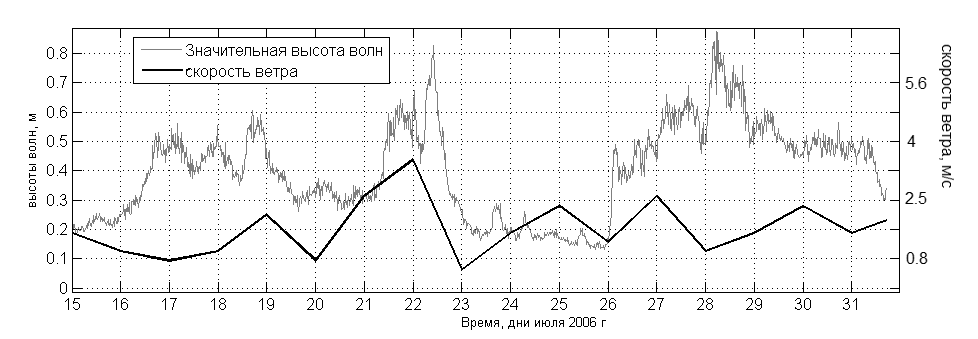
\includegraphics [width=1\linewidth] {hs_windSpeed.png}
  \caption{График высот значительных высот волн(серая линия), расчитанных с использованием негидростатической поправки, по данным полученным вблизи м. Острый и скорость ветра (черная линия), по архивным данным полученным в ближайшем населенном пункте (Долинск)}
  \label{img:hs_windSpeed}
\end{figure}
\FloatBarrier

Необходимо отметить, что значительная высота волны внутри одной группы датчиков, вообще говоря, не является одинаковой. На рис. \ref{img:pdfHsIzm} показаны рассчитанные плотности распределения значительных высот волн на датчиках вблизи озера Изменчивое, показанных на рис. \ref{img:mapIzmenchivoe}. При этом расстояние между датчиками составляет 100 - 700 м. Видно, что слабое волнение весьма неоднородно и пики распределений на каждом датчике различаются. В то же время в случае умеренного волнения (значительная высота волны больше 0.6 м) волнение распределено более равномерно. На рис. \ref{img:pdfHsIzm} отмечается слабое проявление второго пика (0.5 м и 0.7 м), существенно слабее основного(0.15 м). Это можно объяснить тем, что режим волнения в рассматриваемом месте представляет собой суперпозицию двух различных компонент: локальный (прибрежный) режим волнения, возбуждаемого непосредственно в данном бассейне, и совокупность волновых составляющих, приходящих из открытого моря. Подобные типы распределений встречаются и в других работах, описывающих статистику волн в других морях \cite{Soomere_2011}.

\begin{figure} [ht]
  \center
  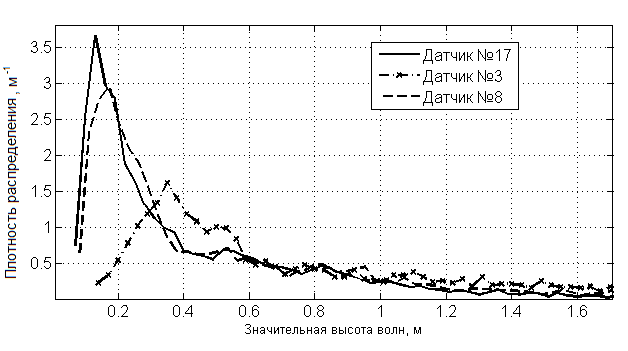
\includegraphics [width=1\linewidth] {pdfHsIzm.png}
  \caption{Плотность распределения вероятности значимых высот волн по записям, полученным в районе о. Изменчивое, содержащим около 1 млн. волн}
  \label{img:pdfHsIzm}
\end{figure}
\FloatBarrier

Для получения распределений высот элементарных волн их высоты $h$ нормировались на значительную высоту волны $H_S$ в каждой двадцатиминутной выборке, а затем по полной записи рассчитывалось распределение высот волн $F(h/H_S)$. Экспериментальные распределения аппроксимировались распределением Вейбулла

 \begin{equation} \label{eq:commonWeib}
F(h/H_S)=1-\exp \left[-b\left(\frac{h}{H_{s} } \right)^{p} \right]
\end{equation}

c параметрами $b$ и $p$. Они сравнивались с распределением Рэлея, справедливым для волн в открытом море \cite{Lopatukhin_1974}

\begin{equation} \label{eq:rayleigh}
F(h/H_S)=1-\exp \left[-2\left(\frac{h}{H_{s} } \right)^{2} \right],
\end{equation}


распределением Форристолла \cite{Forristall_1978}

\begin{equation} \label{eq:forristall}
F(h/H_S)=1-\exp \left[-2.26\left(\frac{h}{H_{s} } \right)^{2.126} \right],
\end{equation}

и распределением Глуховского для волн в море конечной глубины \cite{Glukovsky_2007}

\begin{equation} \label{eq:Glukhovsky}
F(h)=1-\exp \left[-\frac{\pi }{4(1+n/\pi } \left(\frac{h}{\bar{h}} \right)^{\frac{2}{1-n} } \right],
\end{equation}


где $n=\bar{h}/D$,  $\bar{h}$ --- средняя высота волн, и $D$ –-- глубина.
Методики оценок параметров распределений описаны в работах \cite{Davidan_1978} \cite{Lopatukhin_1974} и использованы в настоящей работе. Подбор параметров распределений Вейбулла осуществлялся с помощью метода наименьших квадратов. Согласованность теоретических и эмпирического распределений оценивалось с помощью критерия Пирсона или критерия $\chi^2$ , с уровнем значимости $\alpha=0.01$. Это означает что  На рис. \ref{img:cdfIzmenchivoe} и \ref{img:cdfVzmorie} показаны рассчитанные распределения высот волн для датчиков вблизи оз. Изменчивое и п. Взморье и их аппроксимации. Экспериментальные данные аппроксимированы распределением Вейбулла \eqref{eq:commonWeib} с $b = 1.989$ и $p = 2.216$ (оз. Изменчивое) и  $b = 1.995$ и $p = 2.219$ (п. Взморье).
\begin{figure} [ht]
  \center
  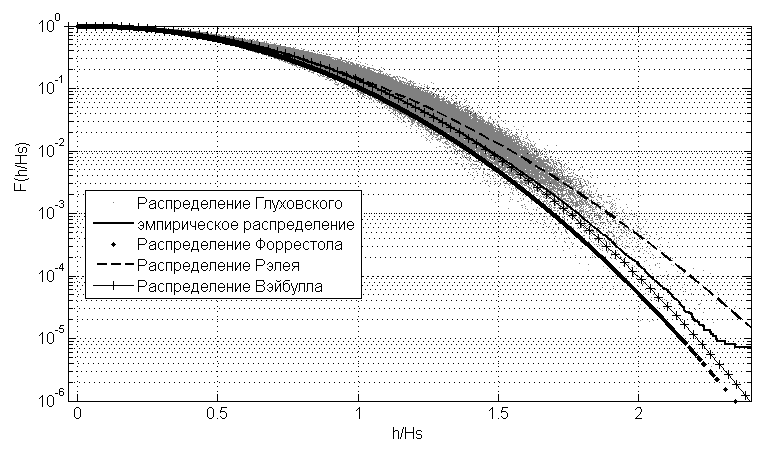
\includegraphics [width=1\linewidth] {cdfIzmenchivoe.png}
  \caption{Функция распределения высот волн $F(h/H_S)$ по записи, полученной в районе оз. Изменчивое, содержащей 1.1 млн. волн}
  \label{img:cdfIzmenchivoe}
\end{figure}
\FloatBarrier

\begin{figure} [ht]
  \center
  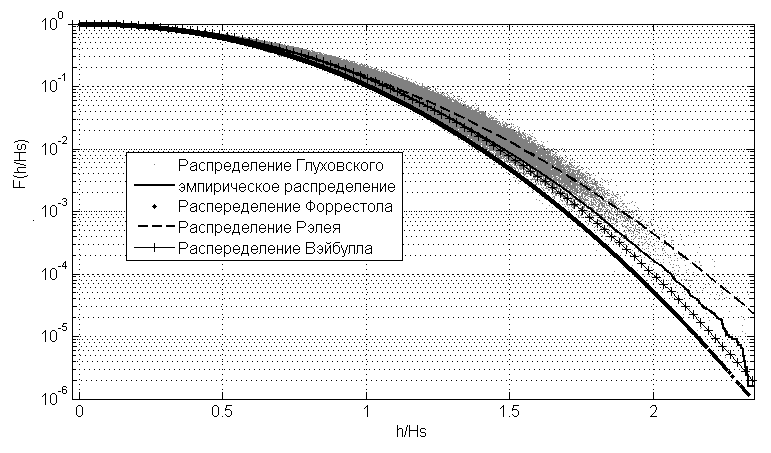
\includegraphics [width=1\linewidth] {cdfVzmorie.png}
  \caption{Функция распределения высот волн $F(h/H_S)$ по записи, полученной в районе оз. Взморье, содержащей 1 млн. волн}
  \label{img:cdfVzmorie}
\end{figure}
\FloatBarrier

Как видно из рис. \ref{img:cdfIzmenchivoe}-\ref{img:cdfVzmorie} распределение Рэлея недостаточно хорошо описывает хвосты функции распределения ($h/H_S > 1.5$), существенно завышая их. Распределения Фористола в целом хорошо описывает эмпирическое распределение (для $h/H_S < 2$), небольшое расхождение присутствует только в области хвостов, соответствующих вероятности появления волн-убийц. Форма распределения Глуховского зависит от средней высоты волны, поэтому на рис. \ref{img:cdfIzmenchivoe} представлено семейство кривых  соответствующих различным режимам погоды. Видно что разнообразие формы распределений при этом достаточно широко, поэтому для оценки распределений высот волн образовавшихся образовавшихся при различных режимах волнених, распределение Глуховского не очень подходит. Наиболее же близко эмпирическое распределение высот волн на юго-восточном побережье о.Сахалин аппроксимирует распределение Вэйбулла \eqref{eq:commonWeib} с параметрами $b = 1.99$ и $p = 2.216$. При значениях $h/H_S>2.3$ начинаются существенные отклонения рассмотренных теоретических распределений от эмпирического. Исследование функций распределения экстремальных волн является самостоятельной задачей, важной для понимания природы волн-убийц. Здесь необходимо вернуться к проблеме пересчета колебаний давления в поле смещений уровня воды, так как линейной теории недостаточно для таких больших волн. Такие исследования предполагается выполнить в дальнейшем.

\subsection{Период волн}
Периодом волн будем называть временную дистанцию, между пересечениями неподвижной точки двумя последовательными гребнями \cite{Davidan_1988}. Существует также метод подсчета периода волн, как времени между последовательными пересечениями нулевого уровня снизу вверх, но подобный метод подсчета связан с большей погрешностью при подсчете, поскольку линию пересечения нулевого уровня необходимо рассчитывать интерполяционными методами.

В работах \cite{Lopatukhin_1974}, \cite{Davidan_1978} (ссылка на давидана) показано, что период ветровых волн и зыби, состоящей из одной волновой системы, хорошо описывается законом Вейбулла с параметром формы $k=3$

\begin{equation} \label{eq:ditribPeriod}
F\left(\tau \right)={\exp  \left(-A{(\tau /\overline{\tau })}^k\right),\ \ где\ A=\Gamma^k(\frac{1}{k}+1)\ }
\end{equation}

В работе показано \cite{Lopatukhin_1974}, что распределение справедливо независимо от способа определения периодов волн по волнограмме: по вершинам, подошвам или по пересечению средней волновой линии.

Такая аппроксимация относится к ветровым волнам и зыби; если волновое поле состоит из нескольких систем волн с различными средними периодами, то $F\left(\tau \right)$ аппроксимируется суммой двух или трех (в зависимости от количества волновых систем) распределений Вейбулла. Смешанное распределение можно записать в виде

\begin{equation} \label{eq:distribStaff}
F\left(\tau \right)=a_1F\left({\tau }_1\right)+a_2F\left({\tau }_2\right)+a_3F({\tau }_3) ,
\end{equation}
где $a_i$ -- весовые множители (такие что $\sum{a_i=1}$), показывающие вклад каждой волновой системы в распределение $F\left(\tau \right)$ \cite{Lopatukhin_1974}.

На рис. \ref{img:pdfPeriodVzmorie} и \ref{img:pdfPeriod_Reg} представлены характерные графики плотностей распределения периодов волн, построенных на основе натурных наблюдений волнения.

\begin{figure} [ht]
  \center
  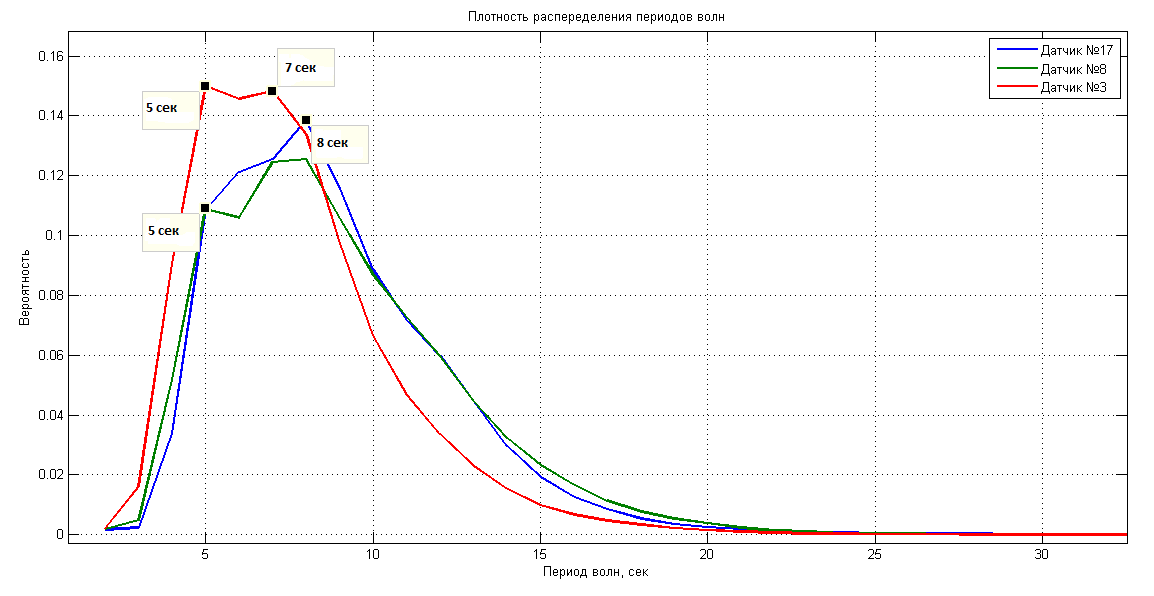
\includegraphics [width=1\linewidth] {pdfPeriodVzmorie.png}
  \caption{Плотность распределения вероятностей периодов волн для записей, полученных вблизи оз. Изменчивое 2007 г.}
  \label{img:pdfPeriodVzmorie}
\end{figure}
\FloatBarrier

По рис. \ref{img:pdfPeriodVzmorie} видно, что наиболее вероятный период волн, на всех трех приведенных реализациях, составляет 8 с. Отличие заметно на записи с датчика №3, который расположен ближе остальных к берегу, график демонстрирует, что там больше встречаемость волн с меньшими периодами, что связано с трансформацией волнения при подходе к берегу.

\begin{figure} [ht]
  \center
  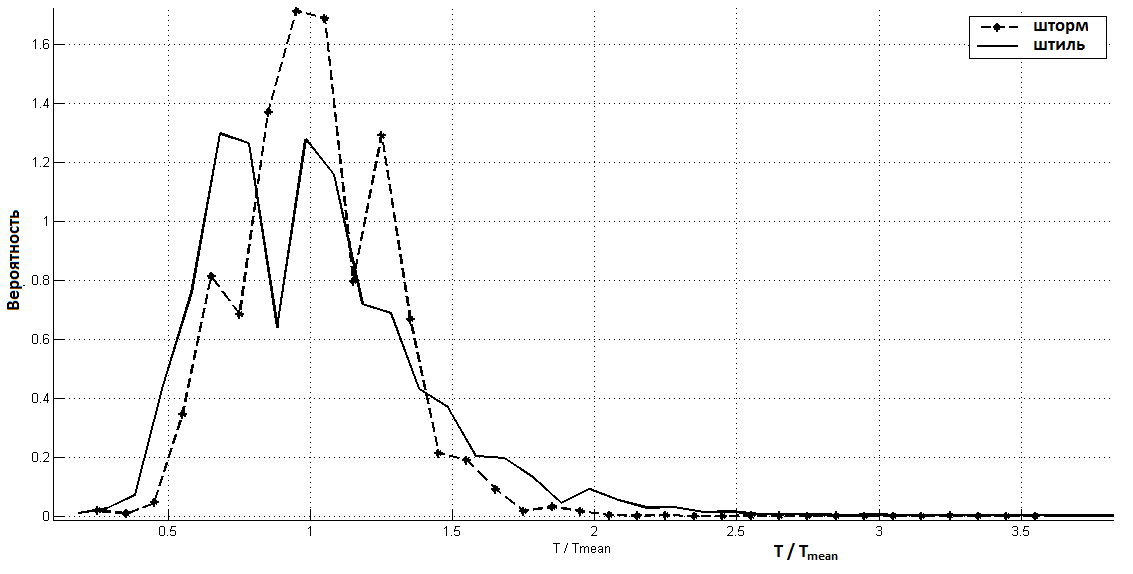
\includegraphics [width=1\linewidth] {pdfPeriod_Reg.png}
  \caption{Плотность распределения периодов волн при различных режимах волнения по датчику №17, расположенному в районе оз.Изменчивое.}
  \label{img:pdfPeriod_Reg}
\end{figure}
\FloatBarrier

На рис. \ref{img:pdfPeriod_Reg} представлены маргинальные распределения относительных периодов волн $F(\tau /\overline{\tau })$ при различных режимах волнения - шторм и спокойная погода. Видно что распределения сильно не похожи друг на друга, при различных режимах волнения.
Этим распределение периодов волн очень сильно отличается от распределений относительных высот волн $F(h/H_S)$.

Возможно поэтому оказалось очень трудно аппроксимировать большие ансамбли натурных данных с помощью теоретических распределений \eqref{eq:distribStaff} \eqref{eq:ditribPeriod}.

\subsection{Сравнительная оценка пространственного распределения статистических характеристик}

Ниже приведены некоторые статистические параметры, рассчитанные по данным натурных наблюдений:

\LTXtable{\textwidth}{tblStatisticCharact}

Данная таблица дает представления только о пространственной изменчивости статистических характеристик. Как видно из этой таблицы а также из рисунка 8 наибольшие волны в районе оз.Изменчивое регистрируются на датчике расположенном ближе всего к берегу(400 метров от берега) в то время как на датчике, удаленном от берега на расстояние 900 м и стоящем на примерно такой же глубине 14 метров, наблюдаемые высоты волн меньше более чем в два раза. Возможно, это связано с тем, что точка, где стоял этот прибор, попала в область фокусировки волн. Статистические параметры высот и периодов в районе м.Острый остаются примерно одинаковыми на всех записях. Наиболее частые периоды волн для всех регионов одни и те же, и составляют 5-6 секунд и 8-9 секунд.

В районе поселка Взморье наиболее частые периоды волны составляют 5 и 7 секунд, причем пик 7 секунд является доминирующим в регионе, поскольку 5 секундный пик на некоторых датчиках, проявляется слабо на графике плотности распределения периодов. Также в этом районе очень сильный разброс высот волн, так на датчике удаленном от берега на расстояние более 1 км средняя значимая высота составляет 77 см, в то время как на датчике N37 значимая высота волны составляет 20 см. Это может быть обусловлено тем, что датчик расположен достаточно близко к мысу, который закрывает его высоких волн.

Можно сделать вывод, что высоты волн очень сильно зависят от пространственного расположения датчика, близости к берегу, защищенности мысом, зон фокусировки и т.д., даже больше чем от глубины постановки датчика.

\section{Характеристики ветрового волнения}

Сотрудниками ИМГиГ и НГТУ в июне-сентябре 2008 года были установлены автономные регистраторы волнения и уровня в населенных пунктах от Гонозаводска на юге до Бошняково на севере (рис. \ref{img:windCharact_1}) на глубинах от 2 до 7 метров. Постановка датчиков придонного гидростатического давления осуществлялась преимущественно без использования плавсредств. Приборы опускались со стенок ковшей портпунктов, и закреплялись на береговом кнехте канатом. Аппаратура была снята в конце сентября – начале октября того же года. По окончанию измерений выяснилось, что из-за заводского брака не работали два датчика в Тельновске и один из двух в Шахтерске, с перебоями работали приборы в Чехове и Красногорске, здесь была получена только часть данных. А прибор, установленный в Томари не был обнаружен. Тем не менее, на большинстве станций был получен качественный материал наблюдений продолжительностью около 4 месяцев.

Одновременно с регистрацией волнения, велись наблюдения за атмосферными параметрами, для этого были установлены 2 автоматические цифровые метеостанции WS-200 в Шахтерске и в Горнозаводске. В результате получены 4-месячные ряды значений приземного атмосферного давления и векторов скорости ветра с дискретностью 1 минута.

\begin{figure} [h]
  \center
  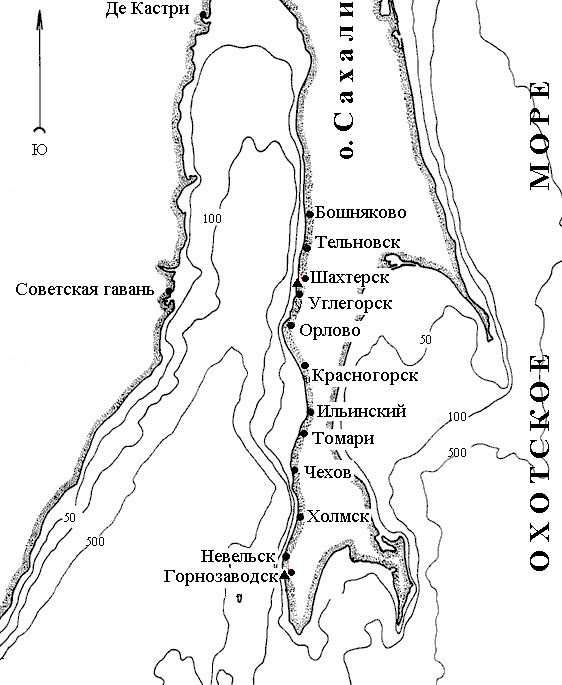
\includegraphics [width=0.7\linewidth] {windCharact_1.png}
  \caption{Схема расположения регистраторов волнения и уровня у западного побережья о.Сахалин. Кружками показано положение автономных цифровых метеостанций, а треугольниками метеостанций.}
  \label{img:windCharact_1}
\end{figure}
\FloatBarrier

Полученные материалы наблюдений были подвергнуты обработке. Данные натурных наблюдений калибровались и приводились к высоте уровенной поверхности, после чего были очищены от прилива и проанализированы на предмет наличия выбросов. Резкие выбросы (их было не много, ни на одном приборе их число не превышало 0,5\%), связанные, по-видимому, с механическим воздействием на корпус прибора, корректировались путем интерполяции по соседним значениям.

Необычно спокойные погодные условия над Татарским проливом Японского моря были отмечены в летний период, а также и в сентябре 2008 года, что в известной мере осложнило анализ материалов экспериментальных измерений. Практически идентичная картина со слабыми непериодическими вариациями уровня отмечена на всем протяженном участке побережья от Горнозаводска до Бошняково.  Можно отметить лишь несколько случаев интенсификации длинноволновых процессов, наиболее выраженных 18-19 июня, 6-7 августа и 3-4 сентября.  Причем интенсивность колебаний несколько различалась на различных участках побережья, но не превышала 50 см. Так, 18-10 июня наибольшие амплитуды волн отмечены на севере (Бошняково, Шахтерск), в южном направлении их величина плавно уменьшалась. Для ситуации 6-7 августа была характерна обратная картина, в начале сентября максимум интенсивности наблюдался в центральной части района, в пос. Ильинский. Наиболее активное волнение было в июне здесь наблюдалось в июне и отмечалось большее количество штормов, по сравнению с другими месяцами.

%В работе [Кабатченко И.М. и др., 2006] представлена методика пересчета спектра пульсаций гидростатического давления к спектру высот поверхностных волн. Соответствующая программа, специально модернизированная под формат имеющихся данных, была предоставлена автором данной методики и использовалась в дальнейшем при расчете характеристик волнении на акватории портов западного побережья Сахалина.
Расчет характеристик волнения (максимальной высоты, периода спектрального максимума волнения) производился с помощью программы представленной \cite{kabat_2007}, расчет выполнялся для последовательных интервалов времени продолжительностью 15 минут.  Это позволило изучить динамику спектральных характеристик ветрового волнения.

Наличие синхронных записей ветрового волнения моря, а также скорости и направления ветра в Шахтерске и Горнозаводске позволило проследить связь этих параметров. При этом важно отметить, что датчик в Шахтерске был поставлен с внешней стороны портового ковша, рядом со стенкой, и был открыт для ветровых волн. В Горнозаводске ситуация была обратная – прибор был установлен внутри достаточно хорошо защищенного ковша, и испытывал влияние только ослабленного волнения.

\begin{figure} [h]
  \center
  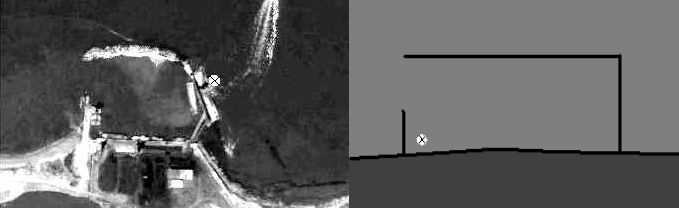
\includegraphics [width=0.7\linewidth] {windCharact_2.png}
  \caption{Расположение регистраторов волнения в порту Шахтерска(слева) и ковше Горнозаводска(справа)}
  \label{img:windCharact_2}
\end{figure}
\FloatBarrier


Были проанализированы данные за июнь 2008 г. - период времени, характеризующийся наибольшим разнообразием волновых режимов. Изучалась эволюция во времени двух характеристик: значимая высота волны и период спектрального максимума.

На рис. \ref{img:windCharact_3} отчетливо видно, что усиление ветра сразу сказывается на изменении характера волнения. Особенно это проявляется в случае сильного ветра 12 июня. Резко увеличивается значимая высота волны - более чем в два раза (с 0.8 до 2 метров). Так же происходит перераспределение энергии из области сравнительно высокочастотного в область низкочастотного ветрового волнения (5-6 с), при высоких скоростях ветра максимум энергии сосредоточен в этом диапазоне. Аналогичные эффекты отмечены и при анализе других случаев усиления ветра в районе п. Шахтерск.

\begin{figure} [h]
  \center
  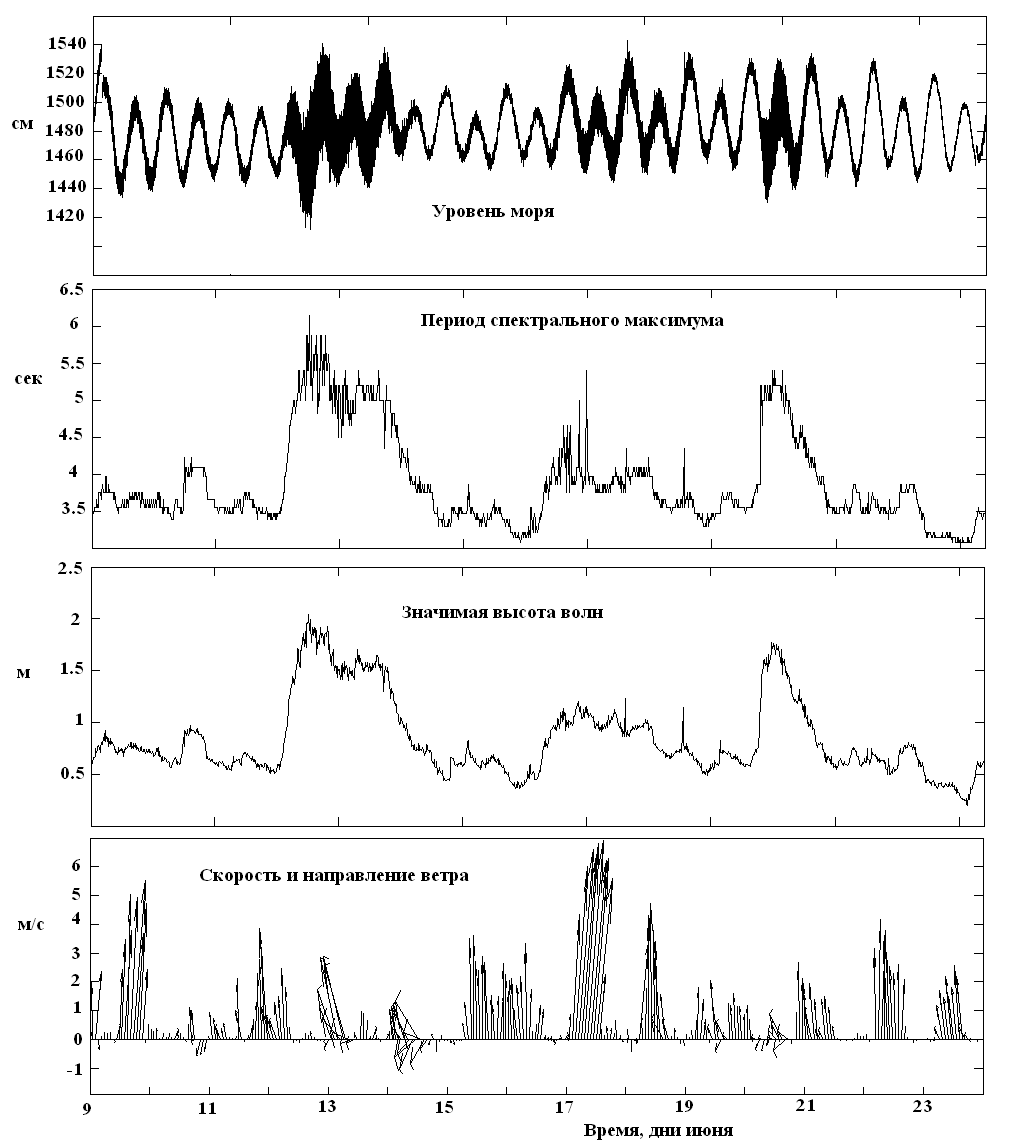
\includegraphics [width=0.7\linewidth] {windCharact_3.png}
  \caption{Изменение характеристик волнения в июне 2008 г. (п. Шахтерск).}
  \label{img:windCharact_3}
\end{figure}
\FloatBarrier

На записи датчика, установленного вблизи п. Горнозаводск, характер волнения несколько иной. Изменение силы ветра мало сказывается на состоянии волнения, происходит это благодаря расположению датчика внутри ковша. Искусственная преграда защищает ковш от проникновения короткопериодных ветровых волн. Поэтому совершенно иные значения имеет период спектрального максимума, среднее значение которого составляет 8 сек, что соответствует диапазону зыби. В п. Шахтерск средний период спектрального максимума равен 3.7 сек, что отвечает диапазону ветрового волнения, обычно преобладающего на акватории Татарского пролива

Значимая высота волн внутри ковша на порядок ниже полученной с внешней стороны -- в п. Горнозаводск она не превышала 20 см, в то время как в п. Шахтерск достигала 2 м. Таким образом, можно сделать вывод о том, что ветровое волнение оказывает слабое злияние на динамические процессы внутри ковша.

\begin{figure} [h]
  \center
  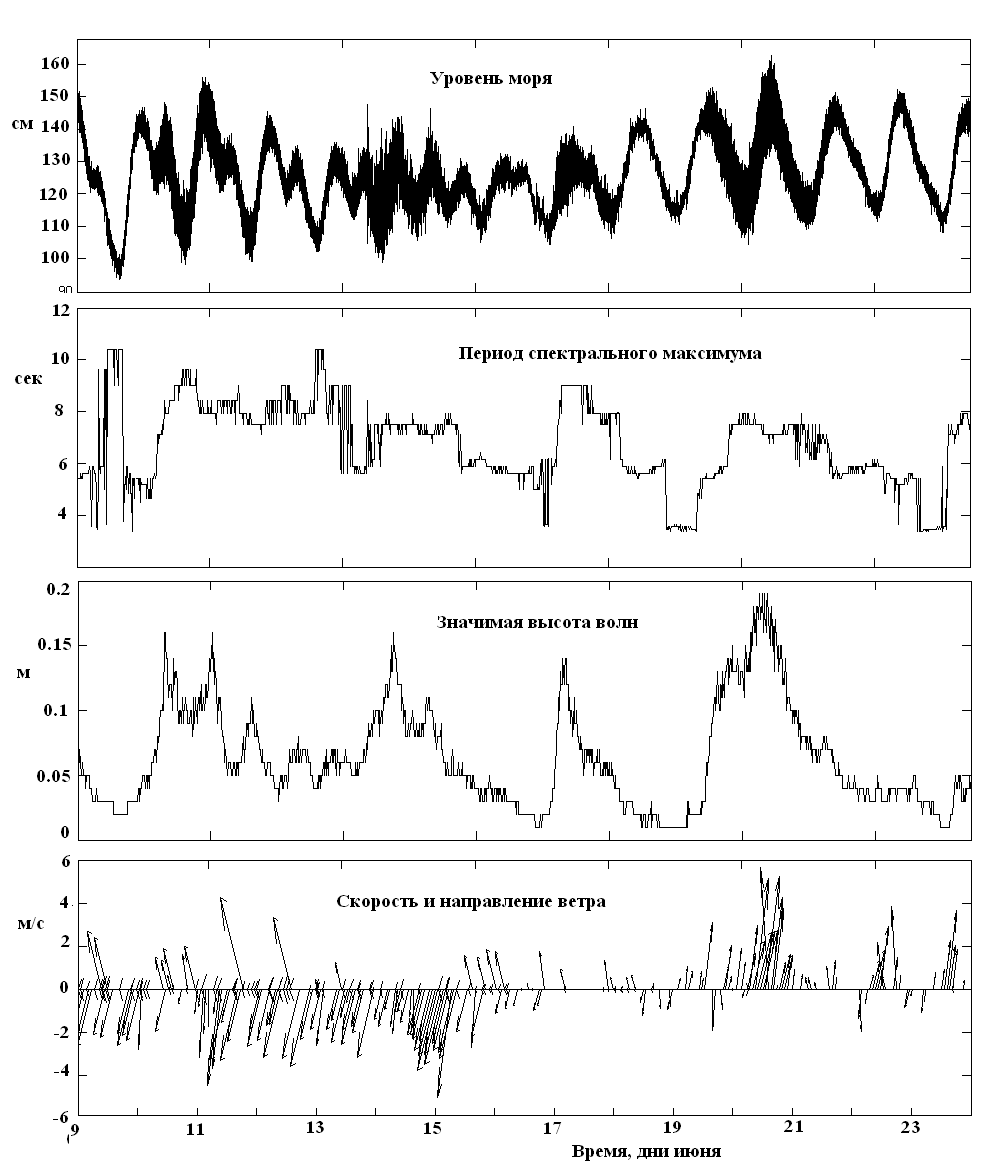
\includegraphics [width=0.7\linewidth] {windCharact_4.png}
  \caption{Изменение характеристик волнения в июне 2008 г. (п. Горнозаводск).}
  \label{img:windCharact_4}
\end{figure}
\FloatBarrier

Рассмотрим подробнее особенности резонансных колебаний в ковше. Для этого проанализируем СВАН-диаграмму, вычисленную по записи волнения, сделанной в г. Углегорск, порт которого имеет четкую прямоугольную форму и поэтому для него легко оцениваются периоды собственных мод. Ковш в г. Углегорск, также как и в п. Горнозаводск, достаточно хорошо защищен от проникновения высокочастотных ветровых волн и на его акватории преобладают более низкочастотные волны.

\begin{figure} [h]
  \center
  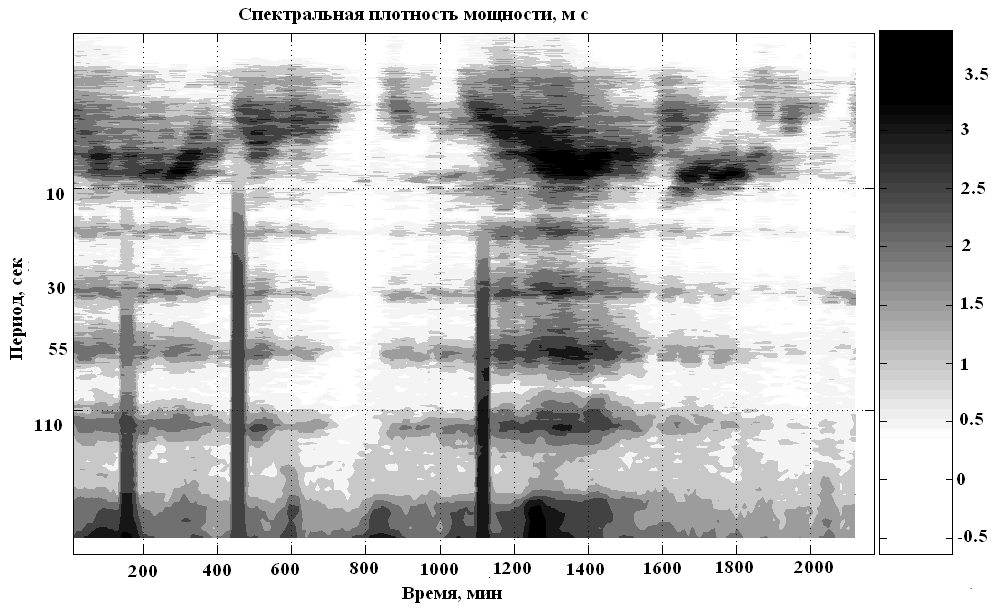
\includegraphics [width=1\linewidth] {windCharact_5.png}
  \caption{Текущий спектр, рассчитанный по записи волнения, сделанной в г. Углегорск.}
  \label{img:windCharact_5}
\end{figure}
\FloatBarrier

Наиболее характерной особенностью текущего спектра является наличие четырех горизонтальных линий с более высокими значениями спектральной амплитуды, которые вероятно, отвечают резонансным модам бассейна. Выделяются максимумы с периодами около 105, 50, 30 и 15 с. Средняя скорость длинных волн на акватории порта составляет около 5 м/с, таким образом, эти периоды неплохо согласуются с оценками периодов одно-и двухузловых продольной и поперечной сейш гавани. Значения выделенных периодов не зависят от исследуемого временного интервала, на протяжении четырех месяцев непрерывных наблюдений они оставались одинаковыми.

Подобная картина характерна для всех портов, в которых проводилась регистрация волнений, разница лишь в значениях выделенных характерных периодов: период нулевой моды меняется для различных портов от 70 (п. Бошняково) до 105 с (г. Углегорск) Эти колебания напрямую связаны с явлением тягуна - периодическими движениями воды в портах, бухтах и гаванях, вызывающими циклические перемещения стоящих у причалов судов. Это существенно затрудняет эксплуатацию их в портах, особенно в процессе погрузки-разгрузки (Гидрометеорология..., 2003).

\textbf{Заключение}

В результате экспериментальных исследований, выполненных на западном побережье о. Сахалин, изучены особенности волнового режима на акваториях портов основных населенных пунктов (за исключением п. Александровск-Сахалинский). Показано, что ковши большинства портпунктов на побережье Татарского пролива хорошо защищены от ветрового волнения. При этом значимая высота волн внутри порта на порядок меньше пс сравнению с внешней акваторией. Происходит также смещение частоты спектрального максимума в низкочастотную область.

Анализ спектрально-временных характеристик показал, что ветровое волнение способно индуцировать резонансные колебания в бухте, что выражается в появлении сейшевых колебаний, с различными характерными периодами, например для г. Углегорск период нулевой моды 105 с, для п. Бошняково - 70 с.

Анализ результатов натурных экспериментов позволил сделать вывод о том, что наибольшую опасность для находящихся в ковшах судов может представлять явление тягуна, связанное с одно- и двухузловыми продольными и поперечными сейшами гаваней. Необходимо также отметить, что тягун проявляется, как правило, при увеличении интенсивности волнения на внешней акватории.

\section{Аномально-большие волны}

\subsection{Соответствие с натурным экспериментом}
Для примера, возьмем записи аномально-больших волн, полученных Специальным конструкторским бюро средств автоматизации морских исследований ДВО РАН в 2009 году у южных берегов острова Сахалин (залив Анива) на мысах залива (мыс Анива) (рис. \ref{img:anivaMap}) \cite{1_Zaits_Pel_Freak_2011}. Измерения проводились с помощью автономных донных регистраторов гидростатического давления \cite{firstResultsSakh_2009}. Дискретность измерений 1 секунда, а глубина постановки прибора на мысу Анива 12 м.

\begin{figure} [h]
  \center
  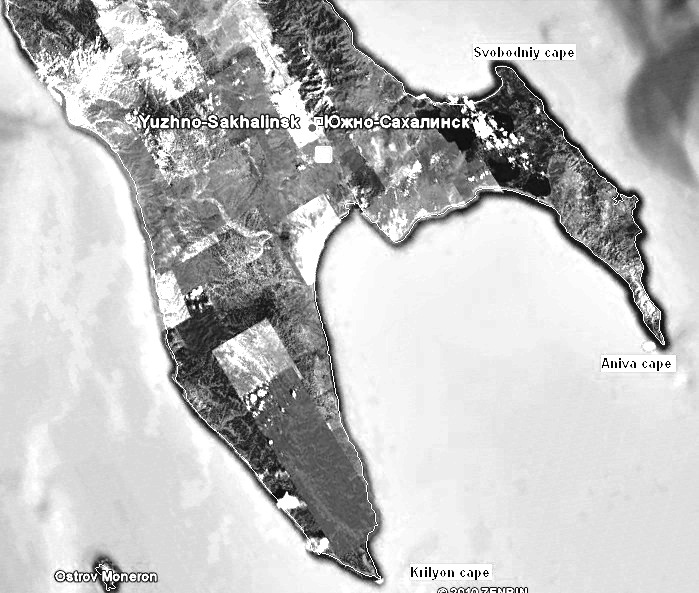
\includegraphics [width=100 mm] {anivaMap.jpeg}
  \caption{Местоположение измерителя волнения в заливе Анива.}
  \label{img:anivaMap}
\end{figure}
\FloatBarrier

Датчик придонного давления регистрирует период и фазу поверхностной волны без изменения, а профиль волны — с некоторыми искажениями, вследствие селективности процесса затухания волн с глубиной (чем меньше длина волны, тем быстрее она затухает). Для коррекции подобных искажений, смещение поверхности восстанавливалось с использованием поправочных коэффициентов, выведенных на основе линейной теории волн \cite{Zasl_Kras_2001},\cite{Huang_Tsai_2008} и подробно рассмотренных в разделе \ref{linTheory}.

Рассмотрим две записи волны-убийцы, представленных на рис. \ref{img:freakAniva_2m} и рис. \ref{img:freakAniva_08m}.

\begin{figure} [h]
  \center
  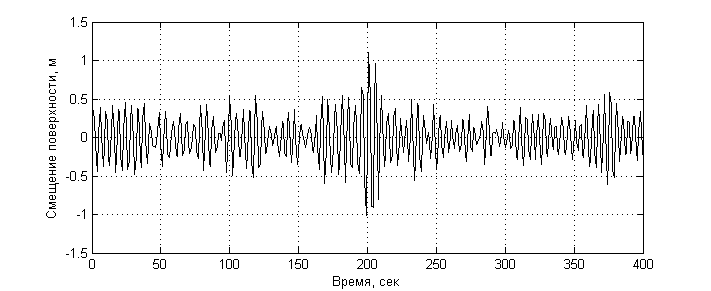
\includegraphics [width=170 mm] {freakAniva_2m.png}
  \caption{Волнограмма с записью волны-убийцы высотой 2.2 метра и превышением значительной высоты волн в 2.42 раза зарегистрирована 19 июля 2009 года в района м.Анива.}
  \label{img:freakAniva_2m}
\end{figure}
\FloatBarrier

\begin{figure} [h]
  \center
  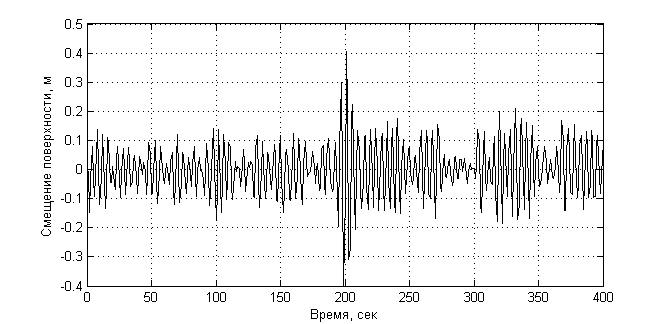
\includegraphics [width=170 mm] {freakAniva_08m.png}
  \caption{Волнограмма волны-убийцы высотой 80 см и превышением значительной высоты волн в 2.54 раза, зарегистрирована 24 июля 2009 года в районе м.Анива.}
  \label{img:freakAniva_08m}
\end{figure}
\FloatBarrier

Первая волна имеет высоту 80 см, а коэффициент $\nu=\frac{H_{max}}{H_S}=2.54$, вторая волна 2.2 метра и $\nu=2.42$ соответственно. Как видно по  волнограммам, эти волны  являются хорошо выраженными волнами-убийцами.  Однако по временной записи колебаний, трудно качественно оценить пространственные характеристики волнения и сравнить их с результатами численного моделирования. Такие характеристики качественно возможно оценить лишь по профилю волнения. В связи с этим  возникает задача восстановления профиля взволнованной поверхности по волнограммам, полученным в одной точке. Решить эту задачу при наличии данных только в одной точке можно лишь в предположении о том, что все волны распространяются в одном направлении.

Основываясь на предположении о том что, если энергия E заключена в диапазоне $S(k)dk$, то столько же энергии будет заключено в диапазоне $S(\omega)d\omega$,
при условии, что $dk$ соответствует $d\omega$ на дисперсионной кривой $\omega(k)$, можно вывести связь пространственного $S(k)$ и временного $S(\omega)$ энергетических спектров:

\begin{equation}\label{eq:relSpectrs}
S(k)=\frac{S(\omega)}{c_gr(\omega)}
\end{equation}

где $с_{gr}(\omega)$ – групповая скорость волн, $k$ – волновое число, связанное с частотой волны $\omega$ дисперсионным соотношением
\begin{equation}\label{eq:dispRelation}
  \omega(k)=sqrt(gkth(kD))
\end{equation}


здесь g – ускорение силы тяжести, D – глубина моря.  В результате, можно восстановить профиль волны по записи волнограммы, но используя случайные фазы. При этом полученный профиль корректно будет использовать лишь для анализа в рамках случайных процессов.

Таким образом, подобная процедура позволит провести сравнительный статистический анализ данных натурных и численных экспериментов, на основе сравнения их геометрических характеристик.

В соответствие с описанной процедурой по временной записи смещения поверхности  моря построим два профиля волнения, один из которых содержит волну-убийцу, а другой в соседние моменты времени до появления аномального события.

\begin{figure} [h]
  \center
  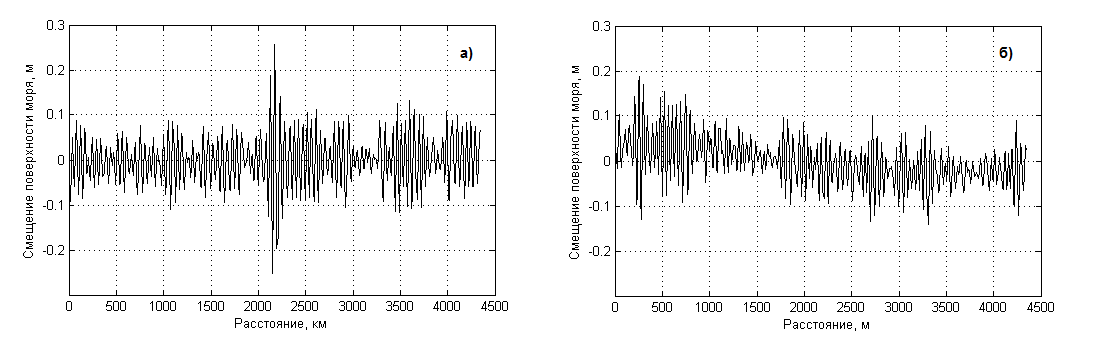
\includegraphics [width=170 mm] {wavegrammFreakNature.png}
  \caption{Профиль поверхности моря, рассчитанный а) по волнограмме, содержащей волну-убийцу б) по волнограмме в соседние моменты времени.}
  \label{img:wavegrammFreakNature}
\end{figure}
\FloatBarrier

По построенным профилям рассчитывалась концентрация геометрических характеристик, описанные выше: длина волн, высота волн, крутизна и кривизна.


\begin{figure} [h]
  \center
  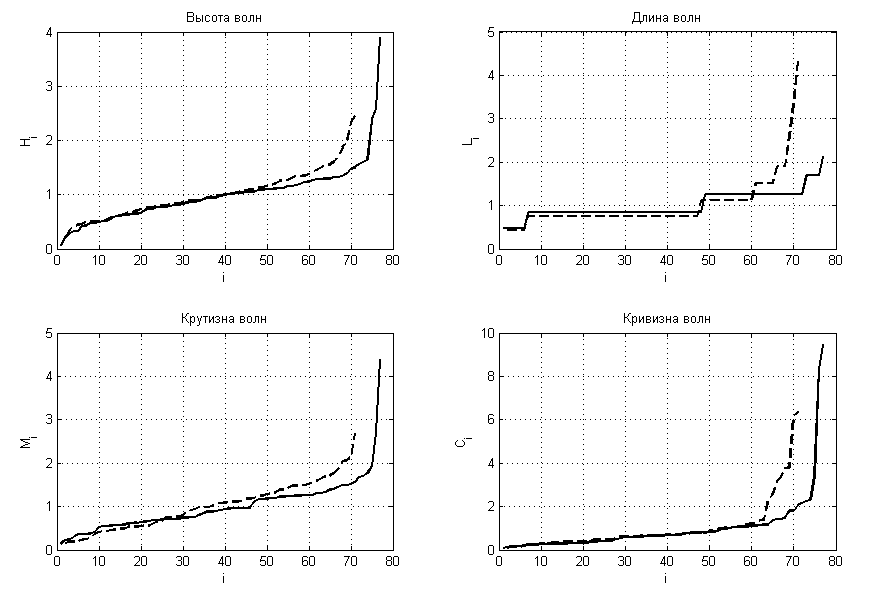
\includegraphics [width=170 mm] {concentrNature.png}
  \caption{Концентрация геометрических характеристик для  волнограммы, содержащей волну-убийцу (сплошная линия) и волнограммы, полученной в соседние моменты времени (пунктирная линия).}
  \label{img:concentrNature}
\end{figure}
\FloatBarrier

Как видно из рис. \ref{img:concentrNature} процессы концентрации характеристик в момент появления волны-убийцы также характерны и для волн, наблюдаемых в открытом море.

Стоит отметить, что расчеты концентрации характеристик по натурным данным имеют на порядок меньшую точность, чем рассчитанные по результатам решения полнонелинейных уравнений ввиду существенных ограничений накладываемых, методом измерения. Однако даже эти данные подтверждают сильную концентрацию всех рассматриваемых геометрических параметров, кроме длины волны. Такое отличие, вероятно связано с недостаточной частотой дискретизации используемого регистратора волнения.

Для выявления характеристик, которые имеют наибольшую концентрацию в момент образования волны-убийцы и наиболее чувствительны к ее появлению, на основе данных натурных наблюдений необходимы дальнейшие исследования.

\section{Заключение}
\clearpage
